\documentclass[titlepage, twoside]{book}
\usepackage{fancyhdr}
\usepackage[italian]{babel}
\pagestyle{fancy}
\fancyheadoffset[RO,LE]{0.4in}
\fancyhead[L]{\leftmark }
\fancyhead[R]{\thepage}
\fancyfoot[C]{\thepage}
\setlength{\headsep}{0.3in}
\fancyfoot[R]{Achille Cannavale}
\usepackage[utf8]{inputenc}
\usepackage[a4paper, total={6in, 10in}]{geometry}
\renewcommand{\thesection}{\arabic{section}}
\usepackage{algorithm}
\usepackage{algpseudocode}

%Per le immagini%
\usepackage{graphicx} 
\usepackage{xcolor}

%Per la Matematica%
\usepackage{mathrsfs,amsmath,amssymb}
\usepackage[makeroom]{cancel}

\usepackage{steinmetz}

%Font Family%
\usepackage{mathptmx}

%Element Font Size%
\usepackage{sectsty}
\sectionfont{\fontsize{18}{20}\selectfont}
\subsectionfont{\fontsize{16}{16}\selectfont}
\subsubsectionfont{\fontsize{12}{12}\selectfont}



%Colori%
\usepackage{empheq}
\usepackage[most]{tcolorbox}

%Per i link nell'indice%
\usepackage{hyperref}
\hypersetup{
    colorlinks,
    citecolor=black,
    filecolor=black,
    linkcolor=black,
    urlcolor=black
}

\newcommand{\vc}[1]{\pmb{\underline{#1}}}
\newcommand{\av}[1]{\mathbb{E}\left[#1\right]}
\newcommand{\rate}[2]{B\log_2\left(1 + \frac{#1}{#2}\right)}


%-------------------------------------------------------%

\begin{document}


\begin{titlepage}
\centering

 \vspace*{\fill}
    {\Huge\bfseries
Reti Wireless\par
}
\vspace{6ex}
{\Large
Riassunto da
\par}

        \vspace{1.5cm}
            
        \textbf{\large Achille Cannavale}
            
        \vfill

        \vspace{0.8cm}

   
\end{titlepage}
\Large

\tableofcontents
\chapter*{Introduzione}
Lo scopo di questa tesi è la progettazione e l'implementazione di un game engine in C++ specializzato nella verifica e nella risoluzione delle collisioni tra corpi rigidi rettangolari. 

L'obiettivo è quello di creare un'architettura solida e performante che possa essere utilizzata per lo sviluppo di giochi 2D di differenti generi, come platformer, metroidvania, arcade e gestionali.
\chapter{Collision Detection}
\section{Separating Axis Theorem}
First of all collect all vertices of both object into a vectort:

\begin{minted}[mathescape, linenos]{c}
std::vector <Vector2f> verticesA = objA->CalculateVertices();
std::vector <Vector2f> verticesB = objB->CalculateVertices();
\end{minted}

Then calculate each normal of all edge, with this relationship:

\[
    normal(\bar{ab}) = \begin{bmatrix}y \; , \; -x \end{bmatrix}
\]

\begin{minted}[mathescape, linenos]{c}
Vector2f CalculateNormal(Vector2f pointA, Vector2f pointB) {
    Vector2f directionVector = pointB - pointA;

    return Vector2f(directionVector.y, -directionVector.x);
}

std::array <Vector2f, 4> CalculateNormals(std::array <Vector2f, 4>& vertices) {
    std::array <Vector2f, 4> normals(vertices.size());

    for (int i = 0; i < vertices.size(); i++) {
        normals[i] = CalculateNormal(vertices[i + 1 % vertices.size()], vertices[i]);
    }
    normals[vertices.size() - 1] = CalculateNormal(vertices[0], vertices[vertices.size() - 1]);
    return normals;
}
\end{minted}

Now, for each normal, we calculate the projection of every vertex on the normal:

\[Projection = vertex \cdot normal\]

And then we calculate the the leastest and the greatest projection for both figures.
Finally `if (maxA < minB || maxB < minA)` there are not collisions.
Else we have a collision and we have to define:

\[axisDepth = \min(maxB - minA,\; maxA - minB)\]

\begin{minted}[mathescape, linenos]{c}
for (Vector2f normal : normals) {
        float minA = INFINITY;
        float maxA = -INFINITY;
        for (Vector2f vertex : verticesA) {
            float proj = Math::Dot(vertex,normal);
            minA = std::min(minA, proj);
            maxA = std::max(maxA, proj);
        }
        float minB = INFINITY;
        float maxB = -INFINITY;
        for (Vector2f vertex : verticesB) {
            float proj = Math::Dot(vertex, normal);
            minB = std::min(minB, proj);
            maxB = std::max(maxB, proj);
        }
        if (maxA < minB || maxB < minA) {

            result.setAreColliding(false);
            result.setCollidingAxis(Vector2f(0, 0));
            result.setDepth(0);
            return result;
        }
        float axisDepth = (std::min(maxB - minA, maxA - minB));
        if (axisDepth < depth) {
            depth = axisDepth;
            result_normal = normal;
        }
    }
\end{minted}
\chapter{Multi Link: Canale SIMO Multi-Utente}
Fino ad ora abbiamo trascurato le interferenze dei segnali trasmessi dagli altri terminali mobili, quindi in questo capitolo ne terremo conto, dato che l'Interferenza Multi-Utente è una caratteristica peculiare delle Reti Wireless.\\

Si dice infatti che i canali wireless sono interference-limited.

\section{Uplink}
Consideriamo K utenti in una cella telefonica che comunicano, allo stesso tempo, con una BS avente L antenne.\\

La BS riceverà la sovrapposizione dei segnali trasmessi dai K utenti:
\begin{equation*}
    \vc{r} = \sum_{k=1}^{K} \sqrt{p_k} \ \vc{h}_k s_k + \vc{n}
\end{equation*}

Supponiamo di voler ricavarci il simbolo trasmesso dall'utente m, possiamo riscrivere così:
\begin{equation*}
    \vc{r} = \underbrace{\sqrt{p_m} \ \vc{h}_m s_m}_{\text{Segnale Utile}}  + \underbrace{\sum_{k \neq m} \sqrt{p_k} \ \vc{h}_k s_k}_{\text{Interferenza Multi-Utente}} + \vc{n}
\end{equation*}

Ed ora elaboriamo il segnale ricevuto con un filtro lineare $\vc{c_m}$:
\begin{equation*}
    y_m = \vc{c}^H_m \vc{r} = \underbrace{\sqrt{p_m} \ \vc{c}^H_m \vc{h}_m s_m}_{\text{Segnale Utile}} + \underbrace{\sum_{k \neq m} \sqrt{p_k} \ \vc{c}^H_m \vc{h}_k s_k}_{\text{Interferenza Multi-Utente}} + \ \vc{c}^H_m \vc{n}
\end{equation*}

Calcoliamo la Potenza del Segnale Utile:
\begin{equation*}
    p_m |\vc{c}^H_m \vc{h}_m|^2 \av{|s_m|^2} = p_m |\vc{c}^H_m \vc{h}_m|^2
\end{equation*}

Ed ora la Potenza dell'Interferenza e del Rumore Termico:
\begin{equation*}
\begin{aligned}
    \av{\left|\sum_{k \neq m} \sqrt{p_k} \ \vc{c}^H_m \vc{h}_k s_k + \ \vc{c}^H_m \vc{n} \right|^2} &= \av{\left|\sum_{k \neq m} \sqrt{p_k} \ \vc{c}^H_m \vc{h}_k s_k \right|^2} + \av{\left| \ \vc{c}^H_m \vc{n} \right|^2} =  \\
    &= \sum_{k \neq m} \av{\left|\sqrt{p_k} \ \vc{c}^H_m \vc{h}_k s_k \right|^2} + \sigma^2 ||\vc{c}_m||^2 = \\
    &= \sum_{k \neq m} p_k \left|\vc{c}^H_m \vc{h}_k  \right|^2 \av{|s_k|^2} + \sigma^2 ||\vc{c}_m||^2 = \\
    &= \sum_{k \neq m} p_k \left|\vc{c}^H_m \vc{h}_k  \right|^2 + \sigma^2 ||\vc{c}_m||^2
\end{aligned}
\end{equation*}

Quindi il SINR dell'utente m sarà:
\begin{equation*}
    SINR_m = \frac{p_m |\vc{c}^H_m \vc{h}_m|^2}{\sum_{k \neq m} p_k \left|\vc{c}^H_m \vc{h}_k  \right|^2 + \sigma^2}
\end{equation*}

Tuttavia con la Ricezione Lineare, da sola, non consente di raggiungere la capacità a causa dell'Interferenza Multi Utente, quindi per ottenerla bisognerebbe usare tecniche di ricezione non-lineari, ma di conseguenza aumenta la complessità.

\subsection{Sum-Rate}
Per misurare le prestazioni globali del sistema in termini di rate si usa:
\begin{equation*}
    R_{sum} = B \sum_{m=1}^K \beta_m \log_2(1 + SINR_m)
\end{equation*}
dove $\beta_m$ è la priorità dell'utente m.

\subsection{Global Energy Efficency e sum-EE}
Per misurare le prestazioni globali del sistema in termini di EE si usa la Global Energy Efficency:
\begin{equation*}
    GEE = \frac{B \sum_{m=1}^K \beta_m \log_2(1 + SINR_m)}{P_c + \sum_{m=1}^K \mu_k \ p_m} 
\end{equation*}
oppure la Sum-EE:
\begin{equation*}
    EE_{sum} = B \sum_{m=1}^K \frac{ \beta_m \log_2(1 + SINR_m)}{\mu_k \ p_m + P_{c,m}} 
\end{equation*}

\subsection{Filtro Adattato (MRC)}
Il Filtro Addattato non è il miglior ricevitore lineare, ma è di sicuro il più semplice da implementare.\\
Sia:
\begin{equation*}
    \vc{c}_m = \vc{h}_m / ||\vc{h}_m||, \forall m = 1,...,K
\end{equation*}

Si cerca di massimizzare la potenza del Segnale Utile, mitigando l'Interferenza Multi-Utente con l'uso di antenne multiple:
\begin{equation*}
\begin{aligned}
      &\textbf{Potenza Interferente} \ \sum_{k \neq m} p_k \left|\vc{h}^H_m \vc{h}_k  \right|^2 = \sum_{k \neq m} p_k \left|\sum_{l=1}^L \vc{h}^*_{m,l} \vc{h}_{k,l}  \right|^2 \\
    &\textbf{Potenza Utile} \ p_m \left|\vc{h}^H_m \vc{h}_m  \right|^2 = p_m \left|\sum_{l=1}^L |\vc{h}^*_{m,l}|^2 \right|^2
\end{aligned}
\end{equation*}

\subsubsection{SINR con Filtro Adattato}

\begin{equation*}
    \begin{aligned}
          SINR_m &= \frac{p_m ||\vc{h}_m||^2}{\sum_{k \neq m} p_k \frac{|\vc{h}^H_m \vc{h}_k |^2}{||\vc{h}_m||^2}+ \sigma^2}
    \end{aligned}
\end{equation*}


\subsection{Zero-Forcing}
Il metodo Zero-Forcing consiste nell'azzerare l'Interferenza Multi-Utente, tuttavia non avremo controllo sulla potenza del Segnale Utile.
\subsubsection{Caso Due Utenti}
Per semplicità supponiamo di avere un sistema con solo due utenti:\\
\begin{equation*}
    y_1 = \underbrace{\sqrt{p_1}\vc{c}_1^H \vc{h}_1 s_1}_{{\text{Segnale Utile}}} + \underbrace{\sqrt{p_2}\vc{c}_1^H \vc{h}_2 s_2}_{{\text{Interferenza Multi-Utente}}} + \underbrace{\vc{c}_1^H \vc{n}}_{Rumore Termico}
\end{equation*}

Per azzerare l'Interferenza Multi-Utente dovremo scegliere $\vc{c}_1$ ortogonale ad $\vc{h}_2$.\\
In particolare fissiamo $\vc{c}_1 = \vc{h}_2^{\bot} / \ ||\vc{h}_2^{\bot}||$, ottenendo:
\begin{equation*}
    y_1 = \sqrt{p_1} \left(\frac{\vc{h}_2^{\bot}}{||\vc{h}_2^{\bot}||}  \right)^H \vc{h}_1 s_1 + \left(\frac{\vc{h}_2^{\bot}}{||\vc{h}_2^{\bot}||}  \right)^H \vc{n}
\end{equation*}

Quindi che abbiamo fatto???\\

Abbiamo proiettato il Segnale Ricevuto $\vc{r}$ lungo una direzione ortogonale al vettore di canale interferente ($\vc{h_2}$).\\ \\

Così facendo l'Interferenza viene azzerata, ma non abbiamo il controllo sulla potenza del Segnale Utile (noise enhacement).\\

Dopo l'applicazione dello Zero-Forcing avremo il seguente SNR:
\begin{equation*}
    SNR_{ZF} = p_1 \frac{|(\vc{h}_2^{\bot})^H \vc{h}_1 |^2}{||\vc{h}_2^{\bot}||^2 \sigma^2} < p_1 \frac{||\vc{h}_1||^2}{\sigma^2}
\end{equation*}
\\

Invece, nel caso in cui avessimo avuto un Canale Noise-Limited, i termini $\vc{h}$ sono meno limitanti rispetto al rumore termico, quindi:
\begin{equation*}
    SNR_{NL} = p_1 \frac{||\vc{h}_1||^4}{||\vc{h}_1||^2 \sigma^2} = p_1 \frac{||\vc{h}_1||^2}{\sigma^2}
\end{equation*}
\begin{center}
    Quindi $SNR_{ZF} < SNR_{NL}$.
\end{center}

\subsubsection{Caso Generale}
In generale il segnale filtrato m-esimo sarà:
\begin{equation*}
    y_m = \vc{c}^H \vc{r} = \sqrt{p_m}\vc{c}_m^H \vc{h}_m s_m + \sum_{k \neq m} \sqrt{p_k}\vc{c}_m^H \vc{h}_k s_k + \vc{c}_m^H \vc{n}
\end{equation*}

Quindi dato che vogliamo porre a zero l'Interferenza Multi-Utente e far rimanere il Segnale Utile:
\begin{equation*}
    \begin{matrix}
    \vc{c}_m^H \vc{h}_1 = 0 \\ \\
    \vc{c}_m^H \vc{h}_2 = 0 \\ 
    \vdots\\ 
    \vc{c}_m^H \vc{h}_m = 1 \\ \\
    \vc{c}_m^H \vc{h}_{m+1} = 0 \\ 
    \vdots \\ 
    \vc{c}_m^H \vc{h}_K = 0
    \end{matrix}
\end{equation*}

I vettori di canale ($\vc{h}$) sono Linearmente Indipendenti $\implies$ il sistema di sopra ammette almeno una soluzione se $L \geq K$.\\

Definiamo $\vc{P}^{1/2} = diag(\sqrt{p_1},...,\sqrt{p_k}), \ \vc{s} = [s_1,...,s_K]^T$, e scriviamo il vettore ricevuto così:
\begin{equation*}
    \vc{r} = \sum_{k=1}^K \sqrt{p_k} \vc{h}_k s_k + \vc{n} = \vc{H} \vc{P}^{1/2} \vc{s} + \vc{n}
\end{equation*}
Definendo poi $\vc{C} = [\vc{c}_1,...,\vc{c}_K]$ e $\vc{y} = [\vc{y}_1,...,\vc{y}_K]^T$ si avrà:
\begin{equation*}
\begin{aligned}
    \vc{y} &= \vc{C}^H \vc{r} = \frac{1}{\vc{H}^H \vc{H}} \ \vc{H}^H  \vc{H} \vc{P}^{1/2} \vc{s} + \frac{1}{\vc{H}^H \vc{H}} \ \vc{H}^H  \vc{n} \\
    &= \vc{P}^{1/2} \vc{s} + \vc{w} = \begin{pmatrix}
    \sqrt{p_1} s_1 \\
     \vdots \\
    \sqrt{p_K} s_K
    \end{pmatrix}
    + \vc{w}
\end{aligned}
\end{equation*}

Quindi come abbiamo detto, la soluzione può essere calcolata SOLO quando $L \geq K$ perchè se così non fosse, la matrice $\vc{H}^H \ \vc{H}$ non sarebbe invertibile!!! \\

Infatti, $\vc{H}^H \ \vc{H}$ ha dimensioni K X K, mentre $\vc{H}$ ha dimensioni L X K.\\
Quindi affinchè $\vc{H}^H \ \vc{H}$ sia invertibile deve verificarsi che $L \geq K$, infatti:
\begin{equation*}
    rg(\vc{H}^H \ \vc{H}) \leq rg(\vc{H}) = min\{L,K\}
\end{equation*}
Mentre il $\vc{w}$ avrà:
\begin{equation*}
    \begin{aligned}
    \av{\vc{w}} &= \frac{1}{\vc{H}^H \vc{H}} \ \vc{H}^H  \av{\vc{n}} = 0 \\
    \av{\vc{w}\vc{w}^H} &= \frac{1}{\vc{H}^H \vc{H}} \ \vc{H}^H \av{\vc{n}\vc{n}^H} \left(\frac{1}{\vc{H}^H \vc{H}} \ \vc{H}^H\right)^H = \\
    &= \sigma^2 \frac{1}{\vc{H}^H \vc{H}} \ \vc{H}^H \vc{H} \ \frac{1}{\vc{H}^H \vc{H}} = \\
    &= \sigma^2 \frac{1}{\vc{H}^H \vc{H}}
    \end{aligned}
\end{equation*}

\subsubsection{SNR ZF}
Il Rapporto Segnale-Rumore dell'utente m è:
\begin{equation*}
    SNR_m^{ZF} = \frac{p_m \av{|s_m|^2}}{\sigma^2 ||\vc{h}_m^+||^2} = \frac{p_m}{\sigma^2 ||\vc{h}_m^+||^2}
\end{equation*}
dove $\vc{h}_m^+$ non è altro che la riga m-esima della matrice $\frac{1}{\vc{H}^H \vc{H}} \ \vc{H}^H$



\subsection{Ricevitore LMMSE}
Il miglior filtro lineare è il ricevitore a Minimo Errore Quadratico Medio (LMMSE).
Consiste nel minimizzare per l'appunto l'errore quadratico medio tra il Simbolo da Stimare e il risultato a valle del filtro:
\begin{equation*}
    MSE_m = \av{|y_m - s_m|^2} = \av{|y_m|^2} + \av{|s_m|^2} - 2\Re\{\av{y_m s_m^*}\}
\end{equation*}
Calcoliamo i singoli termini separatamente:
\begin{equation*}
    \begin{aligned}
    \bullet & \av{|y_m|^2} = \av{y_m y_m^*} = \\
    &= \mathbb{E}[\left(\sqrt{p_m}\vc{c}_m^H \vc{h}_m s_m + \sum_{k \neq m} \sqrt{p_k}\vc{c}_m^H \vc{h}_k s_k + \vc{c}_m^H \vc{n}\right) \cdot \\
    & \cdot \left(\sqrt{p_m} \vc{h}_m^H \vc{c}_m s_m^* + \sum_{i \neq m} \sqrt{p_i}  \vc{h}_i^H  \vc{c}_m s_i^* + \vc{n}^H \vc{c}_m   \right)] = \\
    &= p_m \vc{c}_m^H \vc{h}_m \vc{h}_m^H \vc{c}_m \av{|s_m|^2} + \sum_{k \neq m} p_k \vc{c}_m^H \vc{h}_k \vc{h}_k^H  \vc{c}_m \av{|s_k|^2} + \sigma^2 ||\vc{c}_m||^2 = \\
    &= p_m \vc{c}_m^H \vc{h}_m \vc{h}_m^H \vc{c}_m + \sum_{k \neq m} p_k \vc{c}_m^H \vc{h}_k \vc{h}_k^H  \vc{c}_m + \sigma^2 ||\vc{c}_m||^2 \\ \\
    \bullet & \Re{\left(\av{y_m s_m^*} \right)} = \Re{\left(\av{ \left(\sqrt{p_m}\vc{c}_m^H \vc{h}_m s_m + \sum_{k \neq m} \sqrt{p_k}\vc{c}_m^H \vc{h}_k s_k + \vc{c}_m^H \vc{n}\right) \ s_m^*} \right)} = \\
    &= \sqrt{p_m} \av{|s_m|^2} \Re{(\vc{c}_m^H \vc{h}_m)} = \sqrt{p_m} \Re{(\vc{c}_m^H \vc{h}_m)}
    \end{aligned}
\end{equation*}

Ora calcoliamo il gradiente rispetto a $\vc{c}_m$ dei singoli termini:
\begin{equation*}
    \begin{aligned}
    &\nabla_{c_{m}}\left(p_m \vc{c}_m^H \vc{h}_m \vc{h}_m^H \vc{c}_m\right) = 2p_m\vc{h}_m \vc{h}_m^H\vc{c}_m \\
    &\nabla_{c_{m}} \left(p_k \vc{c}_m^H \vc{h}_k \vc{h}_k^H \vc{c}_m\right) = 2p_k\vc{h}_k \vc{h}_k^H\vc{c}_m \\
    &\nabla_{c_{m}} \left(||\vc{c}_m||^2\right) = \nabla_{c_{m}} \left(\vc{c}_m^H \vc{c}_m\right) = 2\vc{c}_m \\
    &\nabla_{c_{m}} \left(\sqrt{p_m} \Re{(\vc{c}_m^H \vc{h}_m)}\right) = \sqrt{p_m}\vc{h}_m
    \end{aligned}
\end{equation*}
Quindi ricaviamo la condizione di Ottimalità:
\begin{equation*}
    \begin{aligned}
    &\nabla_{c_{m}} MSE_m = 0 \\
    &= \underbrace{\left(p_m\vc{h}_m \vc{h}_m^H\vc{c}_m + \sum_{k \neq m} p_k\vc{h}_k \vc{h}_k^H\vc{c}_k + \sigma^2\vc{c}_m \right)}_{\nabla_{c_{m}} \left(\av{|y_m|^2}\right)} = \underbrace{\sqrt{p_m}\vc{h}_m}_{\nabla_{c_{m}} \left(\Re{\left(\av{y_m s_m^*} \right)}\right)} = \\
    &= \left(p_m\vc{h}_m \vc{h}_m^H + \sum_{k \neq m} p_k\vc{h}_k \vc{h}_k^H + \sigma^2\vc{I}_L \right) \ \vc{c}_m = \sqrt{p_m}\vc{h}_m \\ \\
    & \vc{c}_m = \sqrt{p_m} \left(p_m\vc{h}_m \vc{h}_m^H + \underbrace{\sum_{k \neq m} p_k\vc{h}_k \vc{h}_k^H + \sigma^2\vc{I}_L}_{\vc{R}_m} \right)^{-1} \vc{h}_m = \\
    &= \sqrt{p_m} (p_m\vc{h}_m \vc{h}_m^H + \vc{R}_m)^{-1} \vc{h}_m  \\
    &\text{Usando il Lemma di Inversione delle Matrici:} \\
    & \left(p\vc{x}\vc{x}^H + \vc{M} \right)^{-1} = \vc{M}^{-1} - \frac{p\vc{M}^{-1} \vc{x} \vc{x}^H \vc{M}^{-1}}{1 + p\vc{x}^H \vc{M}^{-1}\vc{x}} \\
    &\text{Otterremo:} \\
    &= \sqrt{p_m} \left(\vc{R}_m^{-1} - \frac{p_m \vc{R}_m^{-1} \vc{h}_m \vc{h}_m^H \vc{R}_m^{-1}}{1 + p_m \vc{h}_m^H \vc{R}_m^{-1} \vc{h}_m} \right) \ \vc{h}_m = \\
    &= \frac{\sqrt{p_m}}{1 + p_m \vc{h}_m^H \vc{R}_m^{-1} \vc{h}_m} \ \vc{R}_m^{-1} \vc{h}_m \implies \vc{R}_m^{-1} \vc{h}_m
    \end{aligned}
\end{equation*}

\subsubsection{SINR dell' LMMSE}
\begin{equation*}
\begin{aligned}
     SINR_m^{LMMSE} &= \frac{p_m |\vc{h}_m^H \vc{R}_m^{-1} \vc{h}_m|^2}{\vc{h}_m^H \vc{R}_m^{-1} \left(\sum_{k \neq m} p_k \vc{h}_k \vc{h}_k^H + \sigma^2 \vc{I}_L \right)\vc{R}_m^{-1} \vc{h}_m } = \frac{p_m |\vc{h}_m^H \vc{R}_m^{-1} \vc{h}_m|^2}{\vc{h}_m^H \vc{R}_m^{-1} \vc{h}_m} = \\ \\
     &= \frac{p_m \vc{h}_m^H \vc{R}_m^{-1} \vc{h}_m \vc{h}_m^H \vc{R}_m^{-1} \vc{h}_m}{\vc{h}_m^H \vc{R}_m^{-1} \vc{h}_m} = p_m \vc{h}_m^H \vc{R}_m^{-1} \vc{h}_m 
\end{aligned}
\end{equation*}


\subsubsection{Massimizzazione del SINR}
Ora cerchiamo di massimizzare il Rapporto Segnale Rumore, ovvero cherchiamo il vettore $\vc{c}_m$ tale che:
\begin{equation*}
\begin{aligned}
    &\max_{c_m} \frac{p_m |\vc{c}_m^H \vc{h}_m|^2}{\sum_{k \neq m} p_k |\vc{c}_k^H \vc{h}_k|^2 +\sigma^2 ||\vc{c}_m||^2} \\
    &= \max_{c_m} \frac{p_m \vc{c}_m^H \vc{h}_m \vc{h}_m^H \vc{c}_m}{\vc{c}_m^H \underbrace{\left(\sum_{k \neq m} p_k \vc{h}_k \vc{h}_k^H  +\sigma^2 \vc{I}\right)}_{\vc{R}_m}\vc{c}_m} = \max_{c_m} \frac{p_m \vc{c}_m^H \vc{h}_m \vc{h}_m^H \vc{c}_m}{\vc{c}_m^H \vc{R}_m \vc{c}_m}
\end{aligned}
\end{equation*}
Se definiamo $\vc{x}_m = \vc{R}_m^{\frac{1}{2}} \vc{c}_m$ avremo:
\begin{equation*}
    \max_{x_m} \frac{p_m \overbrace{\vc{x}_m^H\vc{R}^{-1/2}}^{\vc{c}_m^H}\vc{h}_m \vc{h}_m^H  \overbrace{\vc{R}^{-1/2} \vc{x}_m}^{\vc{c}_m}}{||\vc{x}_m||^2} = \max_{x_m} \frac{p_m |\vc{x}_m^H\vc{R}^{-1/2} \vc{h}_m|^2 }{||\vc{x}_m||^2} = p_m \vc{h}_m^H \vc{R}_m^{-1} \vc{h}_m
\end{equation*}
Che raggiunge il suo massimo per $\vc{x}_m = \alpha \vc{R}_m^{-1/2}\vc{h}_m \implies \vc{c}_m = \alpha \vc{R}_m^{-1}\vc{h}_m$
\begin{center}
    Quindi il Ricevitore LMMSE massimizza il SINR!!
\end{center}


\section{Downlink}
Consideriamo ora la tratta Downlink con:\\
\begin{itemize}
    \item K utenti
    \item Una BS con L antenne
\end{itemize}
La BS trasmetterà la sovrapposizione dei segnali per i K utenti.
\begin{equation*}
    \vc{y} = \sum_{k=1}^K \sqrt{p_k} \vc{q}_k \vc{s}_k
\end{equation*}
con:
\begin{equation*}
    \av{||\vc{y}||^2} = p \sum_{k=1}^K ||\vc{q}_k||^2 = P
\end{equation*}

L'utente m riceverà il segnale:
\begin{equation*}
    r_m = \vc{g}_m^H \left(\sum_{k=1}^K \sqrt{p_k} \vc{q}_k \vc{s}_k \right) + n_m = \sum_{k=1}^K \sqrt{p_k}\vc{g}_m^H\vc{q}_k \vc{s}_k + n_m
\end{equation*}
Dato che vogliamo decodificare il simbolo indirizzato all'utente m, riscriviamo il segnale ricevuto $r_m$ così:
\begin{equation*}
    r_m = \underbrace{\sqrt{p_m}\vc{g}_m^H\vc{q}_m \vc{s}_m}_{\text{Segnale Utile}} + \underbrace{\sum_{k \neq m} \sqrt{p_k}\vc{g}_m^H\vc{q}_k \vc{s}_k}_{\text{Interferenza Multi-Utente}} + \underbrace{n_m}_{\text{Rumore Termico}}
\end{equation*}

Calcoliamo la potenza del Segnale Utile:
\begin{equation*}
    p_m|\vc{g}_m^H\vc{q}_m|^2 \av{|\vc{s}_m|^2} =    p_m|\vc{g}_m^H\vc{q}_m|^2
\end{equation*}

Mentre la potenza dell'Interferenza sommata al Rumore è:
\begin{equation*}
    \begin{aligned}
    \av{\left|\sum_{k \neq m} \sqrt{p_k}\vc{g}_m^H\vc{q}_k \vc{s}_k +n_m \right|^2} &= \av{\left|\sum_{k \neq m} \sqrt{p_k}\vc{g}_m^H\vc{q}_k \vc{s}_k \right|^2} + \av{|n_m|^2} = \\
    &= \sum_{k \neq m} \av{|\sqrt{p_k}\vc{g}_m^H\vc{q}_k \vc{s}_k|^2} + \sigma^2 = \\
    &= \sum_{k \neq m} p_ |\vc{g}_m^H\vc{q}_k|^2 \av{|\vc{s}_k|^2} +\sigma^2 = \\
    &=  \sum_{k \neq m} p_ |\vc{g}_m^H\vc{q}_k|^2  +\sigma^2
    \end{aligned}
\end{equation*}

Quindi il SINR dell'Utente m sarà:
\begin{equation*}
    SINR_m = \frac{p_m|\vc{g}_m^H\vc{q}_m|^2}{\sum_{k \neq m} p_ |\vc{g}_m^H\vc{q}_k|^2  +\sigma^2}
\end{equation*}

Definendo $C_m$ la Capacità del Canale tra l'Utente m e la BS si ha:
\begin{equation*}
    R_m = B\log_2 (1 + SINR_m) \leq C_m
\end{equation*}

\begin{equation*}
    EE_m = \frac{B\log_2 (1 + SINR_m)}{P_{c,m} + \mu_m p_m}
\end{equation*}


\subsection{Maximum Trasmit Combining}
Come abbiamo detto il Filtro Adattato (o MTC) non è il migliore tra i filtri lineari, ma è di sicuro il più semplice e consiste nel massimizzare la potenza del Segnale Utile, mitigando l'Interferenza Multi-Utente con l'uso di antenne multiple.\\
Sia:
\begin{equation*}
    \vc{q}_m = \alpha_m \vc{g}_m, \forall m = 1,...,K
\end{equation*}
\\
\begin{equation*}
    \begin{aligned}
     &\textbf{Potenza Interferente} \ \sum_{k \neq m} p_k |\vc{g}_m^H\vc{q}_k|^2 = \alpha_m^2 \sum_{k \neq m} p_k \left|\sum_{l=1}^L g_{m,l}^* g_{k,l}\right|^2 \\
     &\textbf{Potenza Utile} \  p_m |\vc{g}_m^H\vc{q}_m|^2 = \alpha_m^2 p_m \left|\sum_{l=1}^L |g_{m,l}|^2\right|^2
    \end{aligned}
\end{equation*}

\subsection{Zero-Forcing Beamforming}
Lo Zero-Forcing nel Downlink consiste nel trovare un vettore $\vc{q}_m$ ortogonale a TUTTI i K - 1 canali Interferenti:
\begin{equation*}
    r_m = \sqrt{p_m}\vc{g}_m^H\vc{q}_m s_m + \sum_{k \neq m}\sqrt{p_k} \vc{g}_m^H\vc{q}_k s_k + n_m
\end{equation*}
Imponiamo che:
\begin{itemize}
    \item $\vc{g}_k^H\vc{q}_m=0$ per ogni $k \neq m$
    \item $\vc{g}_k^H\vc{q}_m=1$ per $k = m$
\end{itemize}

Vettorizzando e raccogliendo $\vc{g}_k$:
\begin{equation*}
\begin{aligned}
    \vc{r} &= \begin{pmatrix}
    r_1 \\
    r_2 \\
    \vdots \\
    r_K
    \end{pmatrix} =
    \begin{pmatrix}
    \vc{g}_1^H \left(\sum_{k=1}^K \sqrt{p_k} \vc{q}_k s_k  \right) + n_1 \\
    \vc{g}_2^H \left(\sum_{k=1}^K \sqrt{p_k} \vc{q}_k s_k  \right) + n_2 \\
    \vdots \\
     \vc{g}_K^H \left(\sum_{k=1}^K \sqrt{p_k} \vc{q}_k s_k  \right) + n_K
     \end{pmatrix} = \\
     &= \begin{pmatrix}
      \vc{g}_1^H \\
      \vc{g}_2^H \\
      \vdots \\
      \vc{g}_K^H
     \end{pmatrix} 
     \left(\sum_{k=1}^K \sqrt{p_k} \vc{q}_k s_k  \right) + \begin{pmatrix}
     n_1 \\
     n_2 \\
     \vdots \\
     n_K
     \end{pmatrix} = \vc{G}^H \vc{Q} \vc{P}^{1/2}\vc{s} +\vc{n}
\end{aligned}
\end{equation*}
con $\vc{P}^{1/2} = diag(\sqrt{p_1},...,\sqrt{p_K})$\\ \\
Se ora scegliamo $\vc{Q} = \vc{G}(\vc{G}^H\vc{G})^{-1}$ otteniamo:
\begin{equation*}
    \begin{aligned}
        \vc{r} &=  \vc{G}^H \vc{Q} \vc{P}^{1/2}\vc{s} +\vc{n} = \\
        &= \cancel{\vc{G}^H \vc{G}} \ \cancel{(\vc{G}^H\vc{G})^{-1}}\vc{P}^{1/2}\vc{s} +\vc{n} = \\
        &=\vc{P}^{1/2}\vc{s} +\vc{n} = \begin{pmatrix}
        \sqrt{p_1}s_1 \\
        \vdots \\
        \sqrt{p_K}s_K
        \end{pmatrix}
        + \vc{n}
    \end{aligned}
\end{equation*}

Però per fare ciò, la matrice ($\vc{G}^H\vc{G}$) deve essere invertibile, il che richiede $L \geq K$!!!\\ \\
Quindi è necessario che la BS abbia un numero di antenne almeno uguale al numero degli Utenti Interferenti.

\section{Massive MIMO}
Il Massive MIMO è una delle principali tecniche delle reti 5G e consiste nell'uso di un gran numero di antenne alla BS.\\ \\
Tuttavia comporta un maggiore costo nella costruzione e nell'energia dissipata, ma consente di ottenere prestazioni "virtualmente" uguali ad un canale noise-limited con un Filtro Adattato.\\ \\
Dato che l'Interferenza Multi-Utente diventa trascurabile per L >> K:
\begin{equation*}
\begin{aligned}
        \sum_{k\neq m} \frac{p_k}{||\vc{h}_m||^2} \ |\vc{h}_m^H\vc{h}_k|^2 &= \sum_{k\neq m} \frac{p_k}{||\vc{h}_m||^2} L^2 \left|\frac{1}{L}\sum_{l=1}^L h_{m,l}^* h_{k,l} \right|^2 \approx \\
        &\approx  \sum_{k\neq m} \frac{p_k}{||\vc{h}_m||^2} L^2 |\av{H_m^* H_k}|^2 = 0
\end{aligned}
\end{equation*}
Invece il segnale utile viene preservato:
\begin{equation*}
    \frac{p_k}{||\vc{h}_m||^2}|\vc{h}_m^H\vc{h}_k|^2 =  \frac{p_k}{||\vc{h}_m||^2} \left|\sum_{l=1}^L |h_{m,l}|^2\right|^2 \approx   \frac{p_k}{||\vc{h}_m||^2} L^2 \left|\av{|H_m|^2} \right|^2
\end{equation*}
\chapter{Caduta di Potenziale}
\begin{center}
    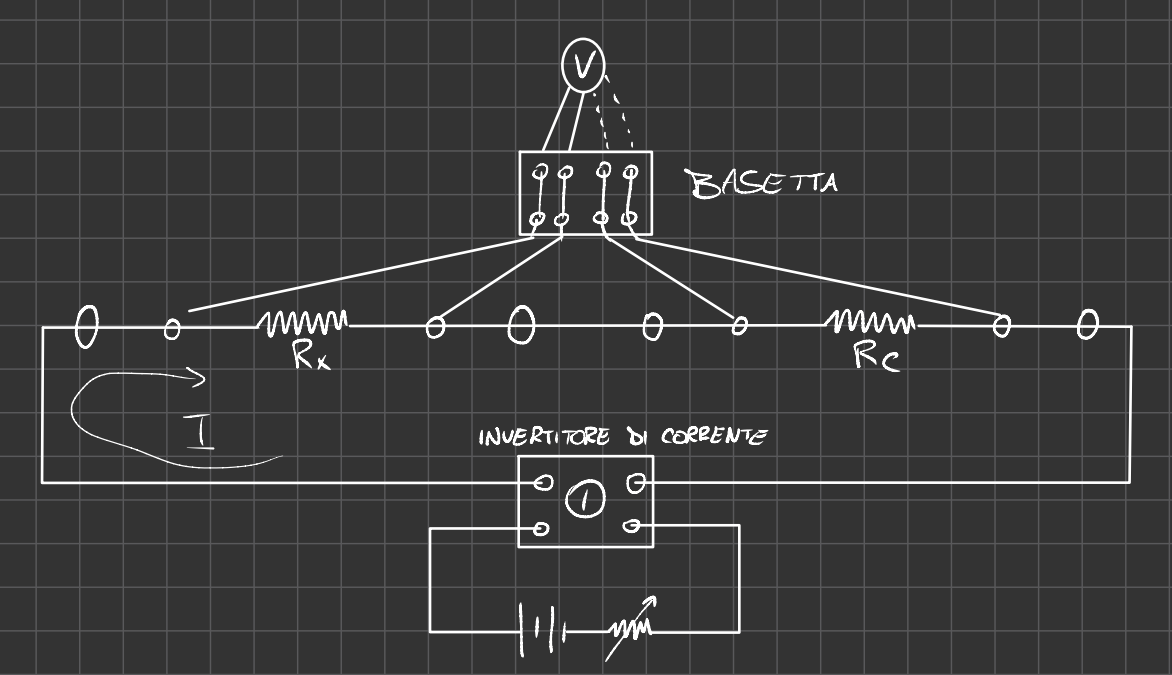
\includegraphics[width=.6\textwidth]{Images/figure43.png}
\end{center}
Questo metodo \textbf{voltamperometrico} viene usato per la misura di \textbf{resistenze di piccolo valore}, eliminando gli \textbf{effetti parassiti} delle \textbf{resistenze di contatto} e delle \textbf{forze elettromotrici di contatto}:
\section{Misurazione}
Vengono eseguite \textbf{quattro misurazioni in serie}:
\begin{itemize}
    \item $V_x$
    \item $V_c$
    \item Cambio verso alla corrente
    \item $-V_c$
    \item $-V_x$
\end{itemize}
\begin{equation*}
    \begin{dcases}
        V_x = R_x I\\
        V_c = R_c I
    \end{dcases}
    \implies V_x = R_x \frac{V_c}{R_c} \implies R_x = R_c \frac{V_x}{V_c}
\end{equation*}
\section{Incertezza}
Essendo:
\begin{equation*}
    V_x \approx V_c \implies \Delta x \approx \Delta c = \Delta
\end{equation*}
Quindi:
\begin{equation*}
    R_x = \frac{\hat{V}_x + \Delta}{\hat{V}_c +\Delta} R_c \implies R_x(\hat{V}_x , \hat{V}_c, \Delta, R_c) = f(...)
\end{equation*}
Calcoliamo l'\textbf{incertezza}:
\begin{equation*}
    \begin{aligned}
        u^2_{R_x} &= \left(\parti{f}{\hat{V}_x}\right)^2 \cdot u^2_{V_x} + \left(\parti{f}{\hat{V}_c}\right)^2 \cdot u^2_{V_c} + \left(\parti{f}{\Delta}\right)^2 \cdot u^2_{\Delta} + \left(\parti{f}{R_c}\right)^2 \cdot u^2_{R_c} =\\
        &=\left(\frac{\cancel{(\hat{V}_c + \Delta)R_c}}{(\hat{V}_c + \Delta)^{\cancel{2}}}\right)^2 \cdot u^2_{V_x} + \left(\frac{(\hat{V}_x - \Delta)R_c}{(\hat{V}_c + \Delta)^2}\right)^2 \cdot u^2_{V_c} + \\
        &+\left(\frac{(\hat{V}_c - \hat{V}_x) R_C}{(\hat{V}_c + \Delta)^2}\right)^2 \cdot u^2_{\Delta} + \left(\frac{\hat{V}_x + \Delta}{\hat{V}_c + \Delta}\right)^2 \cdot u^2_{R_c} =\\
    \end{aligned}
\end{equation*}
Considerando $\Delta \approx 0$ possiamo scrivere:
\begin{equation*}
    = \frac{R^2_c}{\hat{V}^2_c} \cdot u^2_{V_x} + \frac{R^2_c \hat{V}^2_x}{\hat{V}^4_c} \cdot u^2_{V_c} + \frac{\hat{V}^2_x}{\hat{V}^2_c} \cdot u^2_{R_c}
\end{equation*}
Calcoliamo quindi l'\textbf{incertezza} \textbf{relativa} come:
\begin{equation*}
    \dot{u}_{R_x} = \frac{u_{R_x}}{R_x} = \sqrt{\frac{u^2_{V_x}}{\hat{V}^2_x} + \frac{u^2_{V_c}}{\hat{V}^2_c} + \frac{u^2_{R_c}}{R^2_c}}
\end{equation*}
Notiamo quindi che \textbf{più le tensioni sono elevate e meno incertezza su $R_x$ avremo}.
\section{Resistore a 4 morsetti}
In questo tipo di sistema, abbiamo utilizzato resistori a 4 morsetti, dove:
\begin{center}
    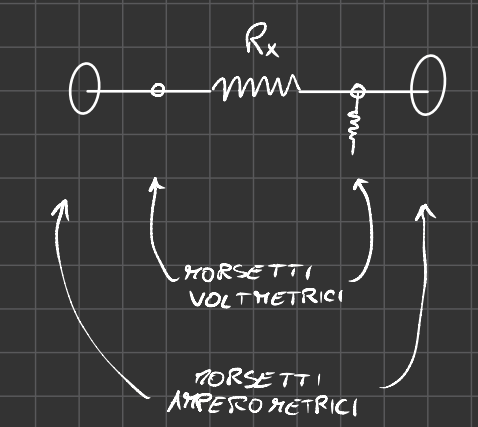
\includegraphics[width=.2\textwidth]{Images/figure44.png}
\end{center}
\begin{itemize}
    \item I due esterni sono detti morsetti amperometrici
    \item I due interni sono detti morsetti voltmetrici
\end{itemize}


\chapter{Adattamenti}
\section{Adattamento con Stub Serie}
\subsection{Metodo 1}
Poniamoci nella situazione in cui vogliamo collegare il carico $Z_l$ sulla linea \textbf{senza} \textbf{perdite}, con \textbf{impedenza} \textbf{caratteristica} $Z_0$:
\begin{center}
    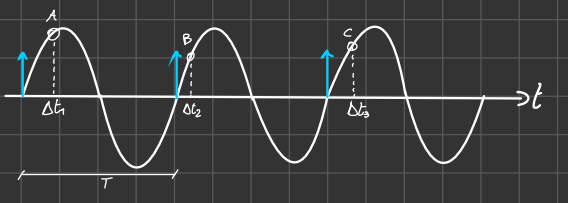
\includegraphics[width=0.8\textwidth]{Images/figure21.png}
\end{center}
Se la colleghiamo direttamente, avremo un \textbf{coefficiente di riflessione} non nullo:
\begin{equation*}
    \Gamma_l = \frac{Z_l - Z_0}{Z_l + Z_0}
\end{equation*}
E un \textbf{ROS} pari a:
\begin{equation*}
    ROS = \frac{1 + |\Gamma_l|}{1 - |\Gamma_l|}
\end{equation*}
Spostandosi lungo la linea, $|\Gamma|$ rimane \textbf{costante}, mentre il \textbf{modulo dell'impedenza} cambia sezione per sezione:
\begin{equation*}
    \frac{Z_0}{ROS} \leq |Z(z)| \leq Z_0 \ ROS
\end{equation*}
E analogamente la \textbf{parte reale dell'impedenza} varia tra:
\begin{equation*}
    \frac{Z_0}{ROS} \leq R(z) \leq Z_0 \ ROS   
\end{equation*}
In particolare esiste una coordinata $z'$ tale che:
\begin{equation*}
    R(z') = Z_0
\end{equation*}
E allo stesso tempo:
\begin{equation*}
    Z(z') = Z_0 + j \underbrace{X(z')}_{X_s}
\end{equation*}
\begin{center}
    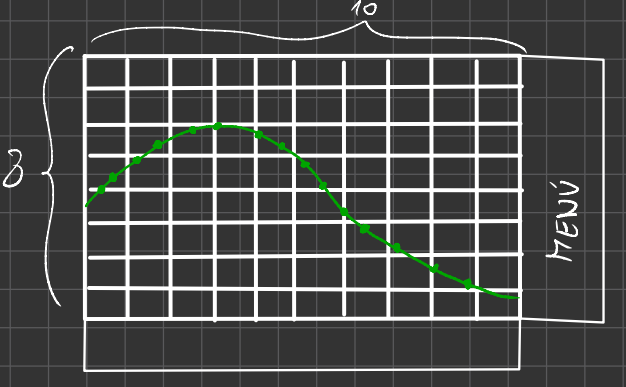
\includegraphics[width=0.7\textwidth]{Images/figure22.png}
\end{center}
\textbf{Ma come posso individuare questa sezione $z'$?\\ \\
}Ricordiamo che:
\begin{equation*}
\begin{aligned}
     Z(z') &= Z_0 \ \frac{1 + \Gamma(z')}{1 - \Gamma(z')} = Z_0 \ \frac{[1 + \Gamma(z')][1 - {\Gamma(z')}^*]}{{|1 - \Gamma(z')|}^2} =\\
     &= Z_0 \ \frac{1 - |\Gamma|^2 + 2j Im\{\Gamma(z')\}}{|1 - \Gamma(z')|^2} =\\
     &=Z_0 \ \frac{1 - |\Gamma|^2 }{|1 - \Gamma(z')|^2} + j Z_0 2 \frac{Im\{\Gamma(z')\}}{|1 - \Gamma(z')|^2}
\end{aligned}
\end{equation*}
Quindi affinchè:
\begin{equation*}
    R(z') = Z_0 \leftrightarrow \frac{1 - |\Gamma|^2 }{|1 - \Gamma(z')|^2} = 1
\end{equation*}
(se $|\Gamma|=1$ la linea è chiusa su una pura reattanza)\\ \\
Se $|\Gamma|<1$:
\begin{equation*}
    \begin{aligned}
    &1 - {|\Gamma|}^2 = {|1 - \Gamma(z')|}^2 = [1 - \Gamma(z')][1 - {\Gamma(z')}^*] = \\
    &= 1 - {\Gamma(z')}^* - \Gamma(z') + {|\Gamma|}^2 = 1 - 2Re\{\Gamma(z')\} + {|\Gamma|}^2
    \end{aligned}
\end{equation*}
Quindi:
\begin{equation*}
    Re\{\Gamma(z')\} = |\Gamma|^2 = |\Gamma_l|^2
\end{equation*}
Ricordando che:
\begin{equation*}
    \begin{aligned}
    \Gamma(z) &= \Gamma(0) e^{2jkz} = \Gamma_l e^{2jkz} = |\Gamma_l| e^{j\varphi_l} e^{2jkz} =|\Gamma_l| e^{j(2kz +\varphi_l)} =\\
    &= |\Gamma_l| \cos(2kz +\varphi_l) + j |\Gamma_l| \sin(2kz +\varphi_l)
    \end{aligned}
\end{equation*}
Quindi sostituendo otterremo:
\begin{equation*}
    Re\{\Gamma(z')\} = |\Gamma_l| \cos(2kz' +\varphi_l) = |\Gamma|^2 \implies \cos(2kz' +\varphi_l) = |\Gamma|
\end{equation*}
Che ha come soluzioni:
\begin{equation*}
    2k z'_n = \frac{4\pi}{\lambda} \pm ar\cos(|\Gamma_n|) - \varphi_l + 2n\pi
\end{equation*}
\begin{equation*}
    \implies z'_n = \pm \frac{ar\cos(|\Gamma_n|)}{2\pi} \frac{\lambda}{2} - \frac{\varphi_l}{2\pi} \frac{\lambda}{2} + n \frac{\lambda}{2} \ \forall n \ : \ z'_n <0
\end{equation*}
Quindi abbiamo trovato le ascisse $z'_n$ in corrispondenza delle quali:
\begin{equation*}
    Z(z'_n) = Z_0 + j Z_0 2 \frac{Im\{\Gamma(z'_n)\}}{|1 - \Gamma(z'_n)|^2}
\end{equation*}
Ricordando anche che:
\begin{itemize}
    \item $1 - |\Gamma_l|^2 = |1 - \Gamma(z_n')|^2 $
    \item $Im\{\Gamma(z'_n)\} = |\Gamma_l| \sin(2kz'_n +\varphi_l) = \pm \sqrt{1 - |\Gamma_l|^2}$
\end{itemize}

Quindi:
\begin{equation*}
    X_s = Im\{Z(z'_n)\} = Z_0 2 \frac{Im\{\Gamma(z'_n)\}}{|1 - \Gamma(z'_n)|^2} =  \pm Z_0 \underbrace{\frac{\sqrt{1 - |\Gamma_l|^2}}{1 - |\Gamma_l|^2}}_{\frac{\sqrt{X}}{X} = \frac{1}{\sqrt{X}}} = \frac{\pm Z_0}{\sqrt{1 - |\Gamma_l|^2}}
\end{equation*}
Quindi per ottenere l'adattamento dobbiamo \textbf{compensare} la $X_s$ inserendo a $z'_n$ una $X_s$ \textbf{uguale} ed \textbf{opposta}:
\begin{center}
    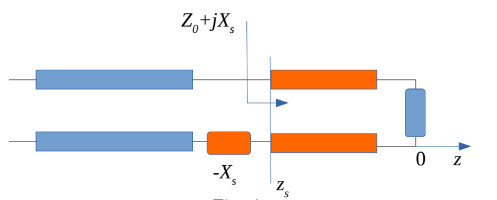
\includegraphics[width=0.7\textwidth]{Images/figure23.png}
\end{center}
La \textbf{reattanza} $X_s$ può essere realizzata con uno \textbf{stub in corto} o con \textbf{uno stub aperto} (es.\ corto):
\begin{center}
    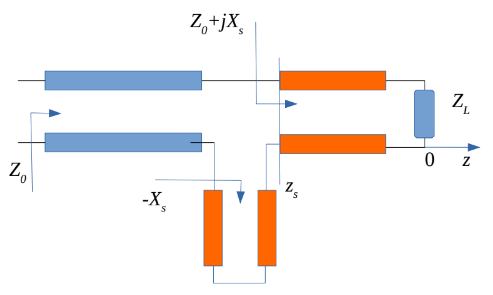
\includegraphics[width=0.7\textwidth]{Images/figure24.png}
\end{center}
\textbf{Ma a che distanza devo mettere lo stub??}\\ \\
\begin{equation*}
    Z(l) = j Z_0 \tan(kl)
\end{equation*}
Quindi pongo:\footnote{La tangente si annulla ogni $n\pi$}
\begin{equation*}
   Z_0 \tan(kl_{stub}) = - X_s
\end{equation*}
\begin{equation*}
  \implies l_{stub} = - atan\left(\frac{X_s}{Z_0}\right) \frac{\lambda}{2\pi} + n \frac{\lambda}{2} \geq 0
\end{equation*}
\subsection{Metodo 2}
Gli stessi risultati li possiamo ottenere con il \textbf{trasporto di impedenza}:\\ \\
Voglio trovare tutte le sezioni in cui \textbf{l'impedenza di carico trasportata ha parte reale $Z_0$}.
\begin{equation*}
    Z(l) = Z_0 \frac{R_l + j Z_0 \tan(kl)}{Z_0 + j R_l \tan(kl)} = Z_0 + j X_s
\end{equation*}
Divido primo e secondo membro per $Z_0$ e numeratore e denominatore per $Z_0$:
\begin{equation*}
    Z'(l) = \frac{R'_l + j t}{1 + j R'_l t} = 1 + j X'_s
\end{equation*}
Dove:
\begin{itemize}
    \item $Z'(l) = \frac{Z(l)}{Z_0}$
    \item $R'(l) = \frac{R_l}{Z_0}$
    \item $X'_s = \frac{X_s}{Z_0}$
    \item $t = \tan(kl)$
\end{itemize}
In particolare:
\begin{equation*}
    \begin{dcases}
    Re\{Z'(l)\} = 1\\
    Im\{Z'(l)\} = X'_s
    \end{dcases}
\end{equation*}
Cerchiamo ora di separare \textbf{parte} \textbf{reale} e \textbf{parte} \textbf{immaginaria}:
\begin{equation*}
    Z'(l) = \frac{(R'_l + j t)(1 - j R'_l t)}{1 +  {R'_l}^2 t^2} = \frac{R'_l - j {R'_l}^2 + jt + R'_l t^2 }{1 + {R'_l}^2 t^2} = 1 + j X'_s
\end{equation*}
Quindi:
\begin{equation*}
    \frac{R'_l + R'_l t^2}{1 +  {R'_l}^2 t^2} = 1
\end{equation*}
\begin{equation*}
    \frac{- {R'_l}^2 t +t}{1 + {R'_l}^2 t^2} = X'_s
\end{equation*}
\textbf{Risolviamo la prima in t}:\\ 
Ricordiamoci però che la vera incognita è l!!\\ \\
Quindi per prima cosa verifichiamo se $t=\infty$, ovvero $l = \frac{\lambda}{4}$ è \textbf{soluzione del problema}:
\begin{equation*}
    t=\infty \implies Z\left(\frac{\lambda}{4}\right) \approx \frac{1}{R'_l} = 1
\end{equation*}
Ma questo può accadere solo se $R'_l = 1$, quindi\textbf{ NON è soluzione.}\\ \\
Procediamo quindi moltiplicando per $1 + {R'_l}^2 t^2$:
\begin{equation*}
    R'_l + {R'_l} t^2= 1 + {R'_l}^2 t^2 \implies ( {R'_l}^2 - R'_l) t^2 = R'_l -1
\end{equation*}
\begin{equation*}
    \implies t^2 = \frac{R'_l -1}{{R'_l}^2 - R'_l} \implies t^2 = \frac{\cancel{R'_l -1}}{R'_l\cancel{({R'_l} - 1)}} = \frac{1}{R'_l} \implies t = \frac{1}{\sqrt{R'_l}}
\end{equation*}
\begin{equation*}
    \implies \tan(kl) = t = \pm \sqrt{\frac{1}{{R'_l}}} = \pm \sqrt{\frac{Z_0}{R_l}}
\end{equation*}
Da questa espressione valuto la l in corrispondenza della quale:
\begin{equation*}
    Z(l) = Z_0 + j X_s
\end{equation*}
Ovvero:
\begin{equation*}
    l = \\arctan\left(\sqrt{\frac{Z_0}{R_l}}\right) \frac{\lambda}{2\pi} + n \frac{\lambda}{2} \geq 0
\end{equation*}
Una volta calcolata la l alla quale vogliamo fare l'adattamento mi ricavo $X_s$:
\begin{equation*}
    \begin{aligned}
    X'_s &= \frac{- {R'_l}^2 t +t}{1 + {R'_l}^2 t^2} = \frac{\pm (1 - {R'_l}^2) \sqrt{\frac{1}{R'_l}}}{1 + R'_l} = \pm \frac{\frac{1 - {R'_l}^2}{\sqrt{R'_l}}}{1 + R'_l} =\\
    &= \pm \frac{1 -{R'_l}^2 }{\sqrt{R'_l} (1 +{R'_l})} = \pm \frac{(1 -{R'_l})\cancel{(1 +{R'_l})}}{\sqrt{R'_l} \cancel{(1 +{R'_l})}} = \pm \frac{1 - {R'_l}}{\sqrt{R'_l}}
    \end{aligned}
\end{equation*}
Quindi:
\begin{equation*}
    X_s = X'_s \cdot \underbrace{Z_0}_{R_0} = \pm \frac{1 - \frac{R_l}{Z_0}}{\sqrt{\frac{R_l}{Z_0}}} \cdot Z_0 = \pm \frac{Z_0 - R_l}{\sqrt{R_l} / \sqrt{Z_0}} = \pm (R_0 - R_l) \cdot \sqrt{\frac{R_0}{R_l}}
\end{equation*}
Questa \textbf{reattanza} va compensata con una \textbf{reattanza} \textbf{uguale} e \textbf{opposta} attraverso uno \textbf{stub serie}:
\begin{equation*}
    X_{stub} = Z_0 \tan(kl_{stub}) = - X_s
\end{equation*}
\begin{equation*}
    kl_{stub} = -\arctan\left(\frac{X_s}{Z_0}\right) + n\pi
\end{equation*}
\begin{equation*}
   \implies l_{stub} = -\arctan\left(\frac{X_s}{Z_0}\right) \frac{\lambda}{2\pi} + n \frac{\lambda}{2} \geq 0
\end{equation*}

\section{Adattamento con Stub Parallelo}
\subsection{Metodo 1}
Nel caso di un \textbf{adattamento} mediante \textbf{stub parallelo} conviene lavorare con le \textbf{ammettenze}.\\
Consideriamo quindi una linea \textbf{senza perdite} con un'\textbf{ammettenza caratteristica} $Y_0 = \frac{1}{Z_0}$ che vogliamo collegare ad un carico di \textbf{ammettenza} $Y_l = \frac{1}{Z_l}$:
\begin{center}
    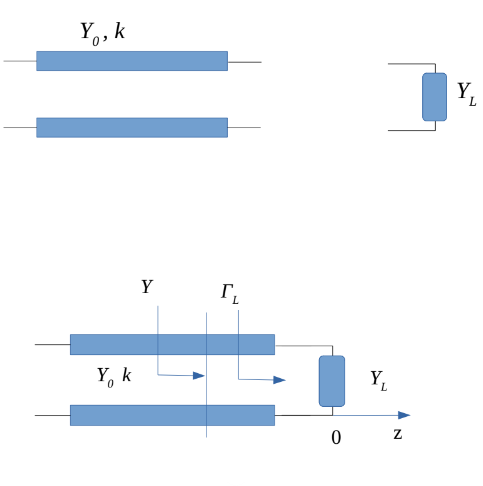
\includegraphics[width=0.7\textwidth]{Images/figure25.png}
\end{center}
Ricordiamo che:
\begin{equation*}
\begin{aligned}
     Y(z') &= Y_0 \ \frac{1 - \Gamma(z')}{1 + \Gamma(z')} = Y_0 \ \frac{[1 - \Gamma(z')][1 + {\Gamma(z')}^*]}{{|1 + \Gamma(z')|}^2} =\\
     &= Y_0 \ \frac{1 - |\Gamma|^2 - 2j Im\{\Gamma(z')\}}{|1 + \Gamma(z')|^2} =\\
     &=Y_0 \ \frac{1 - |\Gamma|^2 }{|1 + \Gamma(z')|^2} - j Y_0 2 \frac{Im\{\Gamma(z')\}}{{|1 + \Gamma(z')|}^2}
\end{aligned}
\end{equation*}
Quindi affinchè:
\begin{equation*}
    Y(z') = G(z') + j B(z') = Y_0 + j B_p \leftrightarrow Y_0 \frac{1 - |\Gamma|^2 }{|1 + \Gamma(z')|^2} = Y_0
\end{equation*}
(se $|\Gamma|=1$ la linea è chiusa su una pura reattanza)
Se $|\Gamma|<1$:
\begin{equation*}
    \begin{aligned}
    &1 - {|\Gamma|}^2 = {|1 + \Gamma(z')|}^2 = [1 + \Gamma(z')][1 + {\Gamma(z')}^*] = \\
    &= 1+ {\Gamma(z')}^* + \Gamma(z') + |\Gamma|^2 = 1 + 2Re\{\Gamma(z')\} + |\Gamma|^2
    \end{aligned}
\end{equation*}
Quindi:
\begin{equation*}
    Re\{\Gamma(z')\} = -|\Gamma|^2 = -|\Gamma_l|^2
\end{equation*}
Ricordando che:
\begin{equation*}
    \begin{aligned}
    \Gamma(z) &= \Gamma(0) e^{2jkz} = \Gamma_l e^{2jkz} = |\Gamma_l| e^{j\varphi_l} e^{2jkz} =|\Gamma_l| e^{j(2kz +\varphi_l)} =\\
    &= |\Gamma_l| \cos(2kz +\varphi_l) + j |\Gamma_l| \sin(2kz +\varphi_l)
    \end{aligned}
\end{equation*}
Quindi sostituendo otterremo:
\begin{equation*}
    Re\{\Gamma(z')\} = |\Gamma_l| \cos(2kz' +\varphi_l) = -|\Gamma|^2 \implies \cos(2kz' +\varphi_l) = -|\Gamma|
\end{equation*}
Che ha come \textbf{soluzioni}:
\begin{equation*}
    2k z'_n = \frac{4\pi}{\lambda} \pm ar\cos(-|\Gamma_n|) - \varphi_l + 2n\pi
\end{equation*}
\begin{equation*}
    \implies z'_n = \pm \frac{ar\cos(-|\Gamma_n|)}{2\pi} \frac{\lambda}{2} - \frac{\varphi_l}{2\pi} \frac{\lambda}{2} + n \frac{\lambda}{2} \ \forall n \ : \ z'_n <0
\end{equation*}
Che sono le \textbf{ascisse} in cui $G = Y_0$.\\ \\
Ripetendo calcoli analoghi:
\begin{equation*}
    Im\{\Gamma(z'_n)\} = |\Gamma_l| \sin(2kz'_n +\varphi_l) = \pm \sqrt{1 - |\Gamma_l|^2}
\end{equation*}
Quindi:
\begin{equation*}
    B_p = Im\{Y(z'_n)\} = Y_0 2 \frac{Im\{\Gamma(z'_n)\}}{|1 + \Gamma(z'_n)|^2} = \pm Y_0 \frac{\sqrt{1 - |\Gamma_l|^2}}{1 - |\Gamma_l|^2} = \frac{\pm Y_0}{\sqrt{1 - |\Gamma_l|^2}}
\end{equation*}
Quindi ora per ottenere l'\textbf{adattamento} devo compensare la \textbf{suscettanza} $B_p$ con una \textbf{suscettanza} \textbf{uguale} ed \textbf{opposta}, attraverso per esempio uno \textbf{stub parallelo} in corto:
\begin{center}
    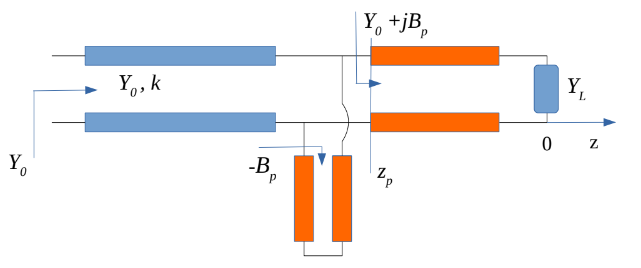
\includegraphics[width=0.7\textwidth]{Images/figure26.png}
\end{center}
\subsection{Metodo 2}
Gli stessi risultati li possiamo ottenere con il \textbf{trasporto di ammettenza}:\\ \\
Voglio trovare tutte le sezioni in cui l'\textbf{ammettenza} di carico \textbf{trasportata} ha \textbf{parte reale} $G_L$.
\begin{equation*}
    Y(l) = Y_0 \frac{Y_l + j Y_0 \tan(kl)}{Y_0 + j Y_l \tan(kl)} = Y_0 + j B_p
\end{equation*}
Divido primo e secondo membro per $Y_0$ e numeratore e denominatore per $Y_0$:
\begin{equation*}
    Y'(l) = \frac{G'_l + j t}{1 + j G'_l t} = 1 + j B_p
\end{equation*}
Dove:
\begin{itemize}
    \item $Y'(l) = \frac{Y(l)}{Y_0}$
    \item $G'_l = \frac{G_l}{Y_0}$
    \item $B'_p = \frac{B_p}{Y_0}$
    \item $t = \tan(kl)$
\end{itemize}
In particolare:
\begin{equation*}
    \begin{dcases}
    Re\{Y'(l)\} = 1\\
    Im\{Y'(l)\} = B'_P
    \end{dcases}
\end{equation*}
Cerchiamo ora di separare \textbf{parte} \textbf{reale} e \textbf{parte} \textbf{immaginaria}:
\begin{equation*}
    Y'(l) = \frac{(G'_l + j t)(1 - j G'_l t)}{1 + j {G'_l}^2 t^2} = \frac{G'_l - j {G'_l}^2 + jt + G'_l t^2 }{1 + j {G'_l}^2 t^2} = 1 + j B'_P
\end{equation*}
Quindi:
\begin{equation*}
    \frac{G'_l + G'_l t^2}{1 + j {G'_l}^2 t^2} = 1
\end{equation*}
\begin{equation*}
    \frac{- {G'_l}^2 t +t}{1 + {G'_l}^2 t^2}
\end{equation*}
Risolviamo la prima in t:\\ 
Procediamo quindi moltiplicando per $1 + {G'_l}^2 t^2$:
\begin{equation*}
    G'_l + {G'_l}^2 = 1 + {G'_l}^2 t^2 \implies ( {G'_l}^2 - G'_l) t^2 = G'_l -1
\end{equation*}
\begin{equation*}
    \implies t^2 = \frac{G'_l -1}{{G'_l}^2 - G'_l} \implies t^2 = \frac{G'_l -1}{G'_l\cancel{({G'_l} - 1)}} = \frac{1}{G'_l} \implies t = \frac{1}{\sqrt{G'_l}}
\end{equation*}
\begin{equation*}
    \implies \tan(kl) = t = \pm \sqrt{\frac{1}{{G'_l}}} = \pm \sqrt{\frac{Y_0}{G_l}}
\end{equation*}
Da questa espressione valuto la l in corrispondenza della quale:
\begin{equation*}
    Y(l) = Y_0 + j B_p
\end{equation*}
Ovvero:
\begin{equation*}
    l = \arctan\left(\frac{Y_0}{G_l}\right) \frac{\lambda}{2\pi} + n \frac{\lambda}{2} \geq 0
\end{equation*}
Una volta calcolata la l alla quale vogliamo fare l'\textbf{adattamento} mi ricavo $B_p$:
\begin{equation*}
    \begin{aligned}
    B'_p &= \frac{- {G'_l}^2 t +t}{1 + {G'_l}^2 t^2} = \frac{\pm (1 - {G'_l}^2) \sqrt{\frac{1}{G'_l}}}{1 + G'_l} = \pm \frac{\frac{1 - {G'_l}^2}{\sqrt{G'_l}}}{1 + G'_l} =\\
    &= \pm \frac{1 -{G'_l}^2 }{\sqrt{G'_l} (1 +{G'_l})} = \pm \frac{(1 -{G'_l})\cancel{(1 +{G'_l})}}{\sqrt{G'_l} \cancel{(1 +{G'_l})}} = \pm \frac{1 - {G'_l}}{\sqrt{G'_l}}
    \end{aligned}
\end{equation*}
Quindi:
\begin{equation*}
    B_p = B'_p \cdot Y_0 = \pm \frac{1 - \frac{G_l}{Y_0}}{\sqrt{\frac{G_l}{Y_0}}} \cdot Y_0 = \pm \frac{Y_0 - G_l}{\sqrt{G_l} / \sqrt{Y_0}} = \pm (Y_0 - G_l) \cdot \sqrt{\frac{Y_0}{G_l}}
\end{equation*}
Questa \textbf{reattanza} va \textbf{compensata} con una \textbf{reattanza} \textbf{uguale} e \textbf{opposta} attraverso uno \textbf{stub} \textbf{parallelo}:
\begin{equation*}
    B_{stub} = Y_0 co\tan(kl_{stub}) = - B_p
\end{equation*}
\begin{equation*}
    kl_{stub} = -arcotan\left(\frac{B_p}{Y_0}\right) + n\pi
\end{equation*}
\begin{equation*}
   \implies l_{stub} = -arcotan\left(\frac{B_p}{Y_0}\right) \frac{\lambda}{2\pi} + n \frac{\lambda}{2} \geq 0
\end{equation*}


\section{Adattamento Tramite Inverter}
Consideriamo la seguente \textbf{linea senza perdite chiusa su un carico}:
\begin{center}
    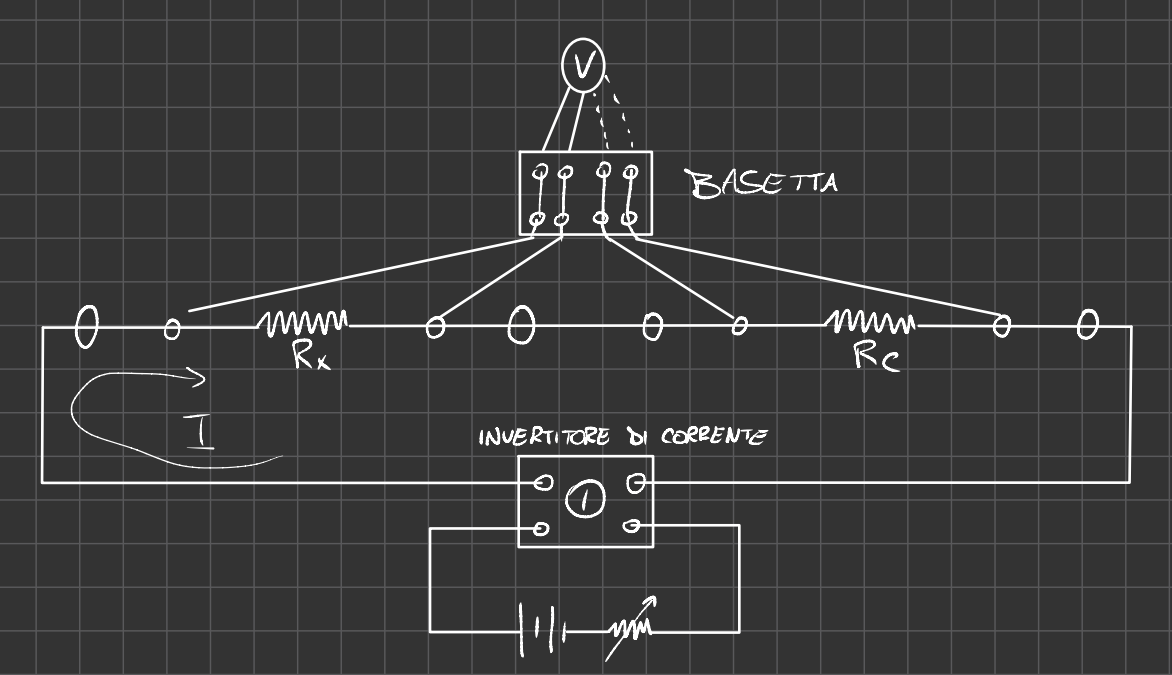
\includegraphics[width=.6\textwidth]{Images/figure43.png}
\end{center}
L'impedenza $Z'_L$ sarà:
\begin{equation*}
    Z'_L = Z_T \frac{Z_L + j Z_T \tan(k_T l)}{Z_T + j Z_L \tan(k_T l)}
\end{equation*}

Nel caso in cui:
\begin{equation*}
    k_T l = \frac{\pi}{2} \implies l = \frac{\lambda_T}{4}
\end{equation*}
Allora:
\begin{equation*}
    k_T l = \left(\frac{\pi}{2}\right) \longrightarrow \infty
\end{equation*}
Quindi va calcolata con il limite:
\begin{equation*}
    Z'_L = \lim\limits_{\tan(k_T l) \longrightarrow \infty} Z_T \frac{Z_L + j Z_T \tan(k_T l)}{Z_T + j Z_L \tan(k_T l)} = \frac{Z_T^2}{Z_L} = Z_T^2 Y_L
\end{equation*}
\textbf{Quindi possiamo dire che il trasporto di un'impedenza di un quarto di lunghezza d'onda lungo una linea da luogo ad un'impedenza proporzionale al reciproco dell'impedenza originale.}




\chapter{Oscilloscopio}
L'\textbf{oscilloscopio} svolge diversi compiti:
\begin{itemize}
    \item \textbf{Acquisire} (campionare  e quantizzare) un segnale
    \item \textbf{Visualizzare} un segnale
    \item \textbf{Misurare}
    \begin{itemize}
        \item Ampiezze
        \item Dominio del tempo
    \end{itemize}
\end{itemize}
Oltre a \textbf{rappresentare} il segnale, è in grado di verificare la presenza di \textbf{disturbi} nel segnare.\\
D'altra parte \textbf{si perde in termini di accuracy}, tuttavia posso lavorare a \textbf{frequenze alte} (10 GHz).
\section{Schema a Blocchi}
\begin{center}
    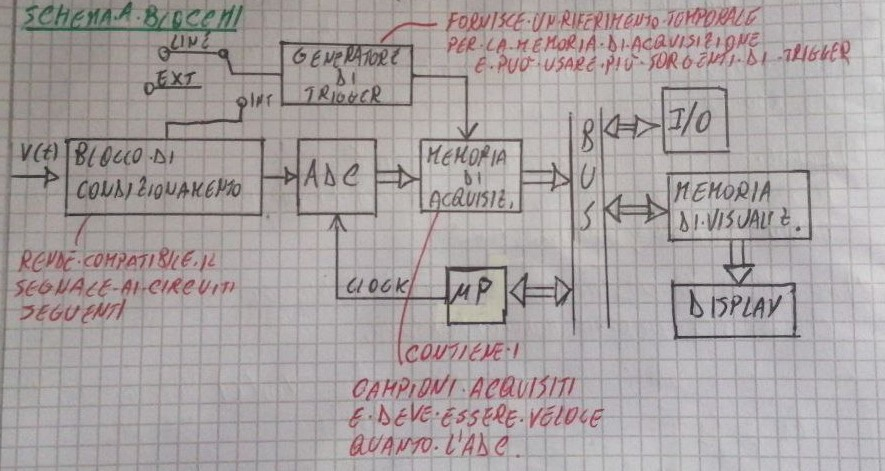
\includegraphics[width=\textwidth]{Images/figure14.jpg}
\end{center}
\section{Blocco di Condizionamento}
\begin{center}
    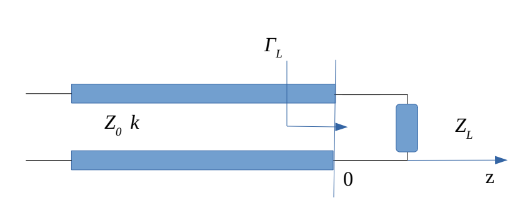
\includegraphics[width=\textwidth]{Images/figure15.png}
\end{center}
\subsection{Accoppiamento}
\begin{itemize}
    \item \textbf{DC}: Non altera il segnale
    \item \textbf{AC}: Passa prima per un condensatore serie che \textbf{filtra} ed \textbf{elimina} la \textbf{componente} \textbf{continua} (offset)
    \item \textbf{Ground}: Collega l'ingresso dell'oscilloscopio a \textbf{ground} per dargli delle condizioni iniziali di riferimento di potenza
\end{itemize}
\subsection{Att/Amp}
\begin{itemize}
    \item \textbf{Attenuatore}: \textbf{attenua} il segnale in accordo con il fondoscala dello strumento.
    \item \textbf{Amplificatore}: \textbf{amplifica} il segnale in accordo con il fondoscala dello strumento.
\end{itemize}
\subsection{Attenuatore Compensato}
\begin{center}
    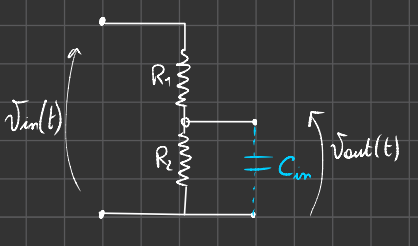
\includegraphics[width=.5\textwidth]{Images/figure16.png}
\end{center}
\begin{equation*}
    V_{out}(t) = V_{in}(t)  \frac{R_2}{R_1 + R_2}
\end{equation*}
\begin{equation*}
    C_{in} = \text{Capacità parassita piccola all'ingresso dell'amplificatore}
\end{equation*}
\begin{equation*}
    V_{out}(t) = V_{in}(t) \cdot \frac{(R_2 // C_{in})}{R_1 + (R_2 // C_{in})} = V_{in}(t)\cdot \frac{\frac{R_2}{j\w C_{in}}}{R_2 + \frac{1}{j\w C_{in}}} \cdot \frac{1}{R_1 + \frac{R_2}{\frac{j\w C_{in}}{R_2 + \frac{1}{j\w C_{in}}}}}
\end{equation*}
Dobbiamo \textbf{annullare} la \textbf{dipendenza} da $\w$ attraverso la \textbf{condizione di compensazione}:
\begin{itemize}
    \item Rendo \textbf{sistematico} ciò che è \textbf{aleatorio} (ovvero $C_{in}$):\\ 
    Metto in \textbf{parallelo} a $C_{in}$ una \textbf{capacità} $C_2$ di valore noto con un ordine di grandezza maggiore.
    \item ho ancora \textbf{dipendenza} da $\w$ quindi aggiungo un'altra \textbf{capacità} $C_1$ da scegliere in modo opportuno.
\end{itemize}
\begin{center}
    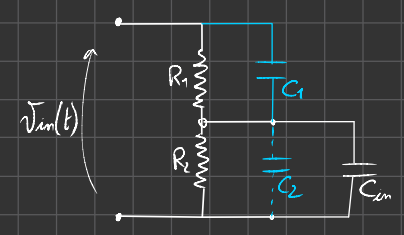
\includegraphics[width=.5\textwidth]{Images/figure17.png}
\end{center}
\begin{equation*}
    V_{out}(t) = \frac{Z_2}{Z_1 + Z_2} \cdot V_{in (t)} \ \text{deve essere indipendente da $\w$}
\end{equation*}
\begin{equation*}
    V_{out}(t) = \begin{dcases}
        \frac{R_2}{R_1 + R_2} V_{in}(t) \quad \w=0\\
        \frac{\frac{1}{j\w C_2}}{\frac{1}{j\w C_1} + \frac{1}{j\w C_2}} \cdot V_{in}(t) = \frac{ V_{in}(t)}{j\w C_2} \cdot \frac{-\w^2 C_1 C_2}{j\w C_1 + j\w C_2} \quad \w \longrightarrow \infty
    \end{dcases}
\end{equation*}
Quindi la \textbf{condizione di compensazione} è:
\begin{equation*}
    R_1 C_1 = R_2 C_2
\end{equation*}
\section{Generatore di Trigger}
Il \textbf{generatore di trigger} deve rispettare alcune esigenze:
\begin{itemize}
    \item Il punto in cui far partire la visualizzazione deve essere arbitrario
    \item La visualizzazione deve consentire di fare misure
\end{itemize}
Al suo interno troviamo:
\begin{center}
    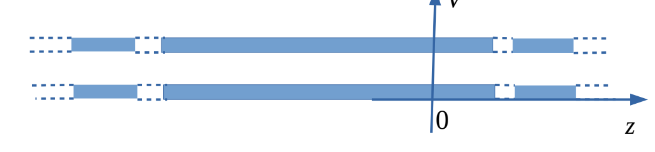
\includegraphics[width=.6\textwidth]{Images/figure18.png}
\end{center}
\section{Memoria di Acquisizione}
La \textbf{memoria} \textbf{di} \textbf{acquisizione} \textbf{circolare} usa una tecnica di memorizzazione \textbf{FIFO}:
\begin{center}
    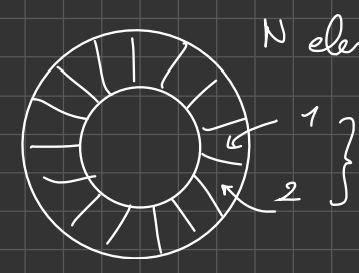
\includegraphics[width=.5\textwidth]{Images/figure19.png}
\end{center}
Esistono due modalità di memorizzazione:
\begin{itemize}
    \item \textbf{Tempo reale }
    \item \textbf{Tempo Equivalente}
    \begin{itemize}
        \item \textbf{Sincorno}
        \item \textbf{Asincrono}
    \end{itemize}
\end{itemize}
\subsection{Tempo Equivalente Sincrono}
Con segnali \textbf{periodici} è possibile evitare di soddisfare \textbf{Nyquist}:
\begin{center}
    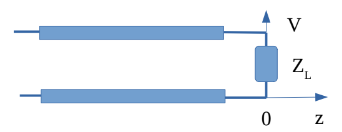
\includegraphics[width=.6\textwidth]{Images/figure20.png}
\end{center}
Dove $\tau = T_c = \left(1 + \frac{1}{M}\right)$.\\
\textbf{In pratica prendiamo un punto per periodo.}
\subsection{Tempo Equivalente Asincrono}
Il campione viene preso in modo \textbf{asincrono} rispetto al \textbf{trigger}
\begin{center}
    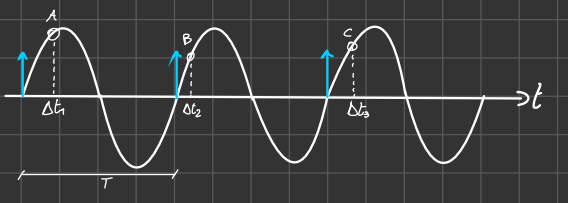
\includegraphics[width=.6\textwidth]{Images/figure21.png}
\end{center}
con $\Delta T_i$ diversi.\\
\textbf{Prendiamo un punto ogni periodo ma a diverse distanze dall'impulso di trigger.
}\section{Display}
\begin{center}
    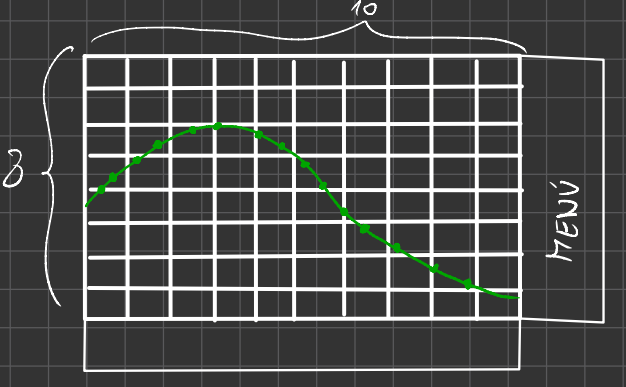
\includegraphics[width=.6\textwidth]{Images/figure22.png}
\end{center}
Attraverso il \textbf{display} è possibile fare alcune \textbf{misurazioni} grazie alle \textbf{griglie} che si trovano sovrapposte al segnale.\\ \\
Un'importante caratteristica di questo \textbf{display}, risiede nel fatto che un classico "\textbf{zoom}" corrisponde ad una diversa \textbf{attribuzione} di \textbf{tempo} o \textbf{tensione} alla \textbf{linea di griglia unitaria.}
\chapter{Risuonatori}
\section{Circuito Risonante Serie}
L'\textbf{impedenza} di un \textbf{circuito LC} è la seguente:
\begin{equation*}
    Z = j\w L + \frac{1}{j\w C} = j \sqrt{\frac{L}{C}} \left(\frac{\w}{\w_0}- \frac{\w_0}{\w}\right)
\end{equation*}
dove $\w_0 = \frac{1}{\sqrt{LC}}$ viene detta \textbf{pulsazione di risonanza}, mentre $\sqrt{\frac{L}{C}}$ è il \textbf{parametro di pendenza}.\\ \\
Alla \textbf{pulsazione di risonanza},\textbf{ l'energia elettrica immagazzinata nella capacità eguaglia l'energia magnetica immagazzinata nell'induttore}, quindi:
\begin{equation*}
    Z(\w_0) = 0
\end{equation*}
Invece per pulsazioni prossime a $\w_0$, usando l'approssimazione di \textbf{Taylor}, vale:
\begin{equation*}
    Z \approx j \sqrt{\frac{L}{C}} \frac{2(\w - \w_0)}{\w_0}, \quad \w \approx \w_0
\end{equation*}

\section{Circuito Risonante Parallelo}
Nel caso del \textbf{parallelo} si ragiona con le \textbf{ammettenze}:
\begin{equation*}
    Y = j \w C + \frac{1}{j \w L} = j \sqrt{\frac{C}{L}} \left(\frac{\w}{\w_0} - \frac{\w_0}{\w}\right)
\end{equation*}
Dove $\w_0 = \frac{1}{\sqrt{LC}}$, in corrispondenza della quale vale che $W_E = W_M$.

\section{Circuito Risonante con Perdite}
In un \textbf{circuito risonante reale} vi è una \textbf{resistenza} (conduttanza) che tiene conto delle \textbf{perdite}.\\ \\
Facciamo l'esempio del \textbf{circuito serie}:
\begin{equation*}
    Z =  j \sqrt{\frac{L}{C}} \left(\frac{\w}{\w_0}- \frac{\w_0}{\w}\right) + R_L
\end{equation*}
Definiamo il \textbf{fattore di merito del circuito} come:
\begin{equation*}
    Q = \frac{\w_0 \cdot W_{EM}}{P_{diss}} = \frac{2 \w_0 L \frac{|I|^2}{4}}{\frac{1}{2} R_L |I|^2} = \frac{\w_0 L}{R_L}
\end{equation*}
Così l'\textbf{impedenza} diventa:
\begin{equation*}
    Z = j \sqrt{\frac{L}{C}} \left(\frac{\w}{\w_0} - \frac{\w_0}{\w}\right) + \frac{\w_0 L}{Q} = j \sqrt{\frac{L}{C}} \left(\frac{\w}{\w_0} - \frac{\w_0}{\w} + \frac{1}{j Q}\right)
\end{equation*}
Analogo discorso per il \textbf{parallelo}:
\begin{equation*}
    Y = j \sqrt{\frac{C}{L}} \left(\frac{\w}{\w_0} - \frac{\w_0}{\w}\right) + G = j \sqrt{\frac{L}{C}} \left(\frac{\w}{\w_0} - \frac{\w_0}{\w} + \frac{1}{j Q}\right)
\end{equation*}

\section{Capacità Filtranti di un Risuonatore}
Se colleghiamo un \textbf{risuonatore serie} ad un \textbf{generatore ideale di tensione} a pulsazione $\w$, avremo questa \textbf{corrente}:
\begin{squared}[violet]
    I(\w) = \frac{V_0}{j \sqrt{\frac{L}{C}} \left(\frac{\w}{\w_0} - \frac{\w_0}{\w} + \frac{1}{j Q}\right)}
\end{squared}
Per $\w = \w_0$ la corrente avrà il suo \textbf{massimo}:
\begin{equation*}
    I(\w_0) = V_0 Q \sqrt{\frac{C}{L}}
\end{equation*}
\textbf{A quali pulsazioni il modulo della corrente diminuirà di 3dB??}
\begin{equation*}
    \frac{\w}{\w_0} - \frac{\w_0}{\w} = \pm \frac{1}{j Q}
\end{equation*}
Che ha per soluzioni:
\begin{equation*}
    \w = \pm \frac{1}{2} \left(\frac{\w_0}{Q} \pm \sqrt{\frac{{\w_0}^2}{Q^2} + 4 {\w_0}^2}\right) = \left(\w_0 \sqrt{1 + \frac{1}{4Q^2} } \pm \frac{\w_0}{2Q}\right)
\end{equation*}
Che per $Q >> 1$ fornisce $\w = \pm \left(\w_0 \pm \frac{\w_0}{2Q}\right)$
\\ \\
Analizziamo ora il \textbf{caso di un generatore reale}, con una sua \textbf{resistenza interna} $R_0$:
\begin{equation*}
\begin{aligned}
    Z &= j \sqrt{\frac{L}{C}} \left(\frac{\w}{\w_0} - \frac{\w_0}{\w} + \frac{1}{j Q}\right) + R_0 = j \sqrt{\frac{L}{C}} \left(\frac{\w}{\w_0} - \frac{\w_0}{\w} + \frac{1}{j Q} + \frac{1}{j Q_{ext}}\right ) = \\
    &=j \sqrt{\frac{L}{C}} \left(\frac{\w}{\w_0} - \frac{\w_0}{\w}  + \frac{1}{j Q_{tot}}\right )
\end{aligned}
\end{equation*}
Dove:
\begin{equation*}
    Q_{ext} = R_0 \sqrt{\frac{C}{L}}
\end{equation*}
Dunque:
\begin{equation*}
    Q_{tot} = \frac{QQ_{ext}}{Q + Q_{ext}} = \left(\frac{1}{Q} + \frac{1}{Q_{ext}}\right)^{-1}
\end{equation*}
Quindi si avrà:
\begin{squared}[violet]
     I(\w) = \frac{V_0}{j \sqrt{\frac{L}{C}} \left(\frac{\w}{\w_0} - \frac{\w_0}{\w} + \frac{1}{j Q_{tot}}\right)}
\end{squared}
\begin{equation*}
    I(\w_0) = V_0 Q_{tot} \sqrt{\frac{C}{L}}
\end{equation*}
E analogamente a prima, \textbf{la pulsazione a 3dB sarà}:
\begin{equation*}
    \w_{3dB} = \pm \frac{\w_0}{2Q_{tot}}
\end{equation*}
\section{Risuonatori a Parametri Distribuiti}
Consideriamo la seguente situazione e poniamo l'origine su uno dei due corti:
\begin{center}
    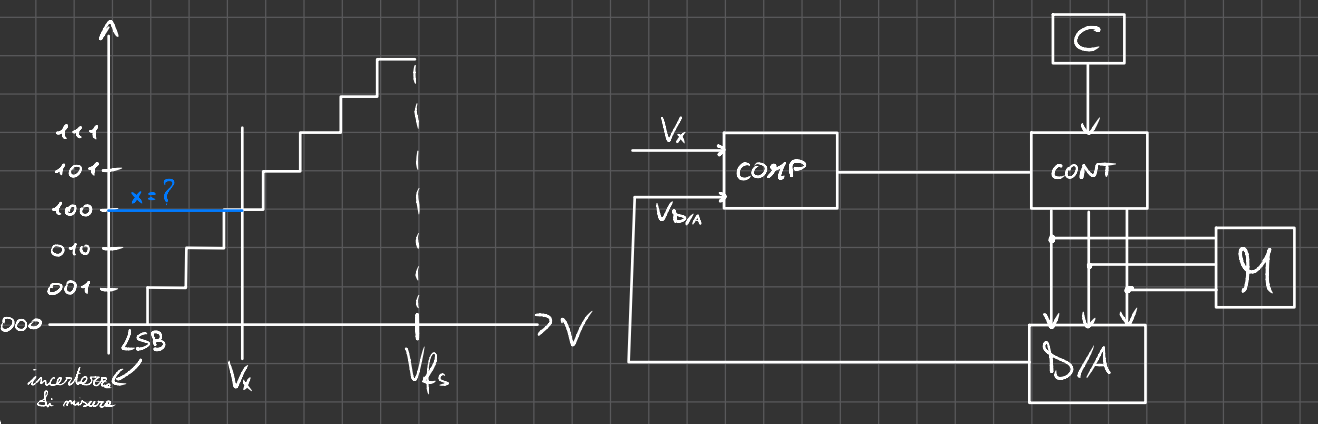
\includegraphics[width=.8\textwidth]{Images/figure28.png}
\end{center}
Avremo i seguenti andamenti di \textbf{tensione} e \textbf{correnti}:
\begin{equation*}
    \begin{dcases}
    V(z) = - j Z_0 I(0) sin(kz)\\
    I(z) = I(0) cos(kz)
    \end{dcases}
\end{equation*}
Mentre l'\textbf{impedenza} sarà:
\begin{equation*}
    Z(z) = - j Z_0 tan(kz) \implies Z(l) = - j Z_0 tan(kl) = Z_R
\end{equation*}
La \textbf{pulsazione di risonanza} è quella in cui $Z = 0$, quindi:
\begin{equation*}
\begin{aligned}
    Z(l) &=  - j Z_0 tan(kl) = 0 \implies tan(\beta l - j \alpha l) \approx \\
    &\approx  tan(\beta l) + \frac{1}{cos^2(\beta l) (-j \alpha l)}
\end{aligned}
\end{equation*}
\textbf{Se le perdite sono piccole} allora:
\begin{equation*}
    \alpha l << 1
\end{equation*}
Quindi:
\begin{equation*}
    Z_R = j Z_0 tan(kl) \approx j Z_0 tan(\beta l) + \frac{Z_0}{cos^2(\beta l)} \alpha l
\end{equation*}
Quindi le\textbf{ pulsazioni di risonanza} sono:
\begin{equation*}
    \w_n: \quad \beta(\w_n) l = (n+1)\pi, \quad n \in N_0
\end{equation*}
In corrispondenza delle quali:
\begin{equation*}
    Z_R = Z_0 \alpha l
\end{equation*}
Quindi ci sono estreme differenze tra \textbf{risuonatori} a \textbf{parametri} \textbf{concentrati} e quelli \textbf{distribuiti}.\\ \\
In un \textbf{risuonatore a parametri concentrati} si ha \textbf{un solo valore di pulsazione di risonanza}, mentre nei \textbf{risuonatori a parametri distribuiti} se ne hanno \textbf{infiniti}.\\ \\
In comune hanno che \textbf{entrambe le impedenze si annullano in risonanza}.\\ \\
Altre analogie le possiamo trovare se analizziamo il comportamento dei due risuonatori in un intorno di ${\w_0}_{(n)}$.\\
Assumiamo che entrambi i \textbf{risuonatori} risuonino a:
\begin{equation*}
    \w_0 = \frac{\pi}{\beta(\w_0)l}
\end{equation*}
Sviluppiamo le due impedenze al primo ordine di \textbf{Taylor}:\footnote{$f(x_0) + \frac{1}{1!}f'(x_0) (x-x_0) $}
\begin{equation*}
    Z'_R \approx \sqrt{\frac{L_0}{C_0}} \left(\frac{\w- \w_0}{2\w_0} - j \frac{1}{Q}\right)
\end{equation*}
\begin{equation*}
    Z_R \approx j Z_0 l \left[\frac{d\beta}{d \w}\right]_{\w=\w_0} (\w - \w_0) + \underbrace{Z_0 \alpha l}_{f(x_0)}
\end{equation*}
Che coincidono se:
\begin{equation*}
    \sqrt{\frac{L_0}{C_0}} = \w_0 \frac{Z_0 l}{2} \left[\frac{d\beta}{d \w}\right]_{\w=\w_0}
\end{equation*}
E se:
\begin{equation*}
    Q = \frac{\w_0}{2\alpha} \left(\left[\frac{d\beta}{d \w}\right]_{\w=\w_0}\right)^{-1}
\end{equation*}
\subsection{Metodo Perturbativo}
Un altro metodo di valutazione è \textbf{l'analisi delle perturbazioni}.\\ \\
Consideriamo una linea \textbf{non dispersiva}, ovvero con i parametri L, R, C, G \textbf{indipendenti} dalla frequenza:
\begin{equation*}
    Z_R = j Z_0 tan(\beta l)
\end{equation*}
\begin{equation*}
    \beta(\w_0) l = (n + 1) \pi, \quad n \in N_0
\end{equation*}
Sviluppiamo $Z_R$ al\textbf{ primo ordine} in $(\w -\w_0) $ e valutiamone il\textbf{ fattore di pendenza}:
\begin{equation*}
    \w_0 \frac{Z_0 l}{2}  \left[\frac{d\beta}{d \w}\right]_{\w=\w_0} = \frac{\w_0 Z_0 l \sqrt{LC}}{2}
\end{equation*}
Per valutare Q scriviamo \textbf{tensione} e \textbf{corrente} lungo la linea:
\begin{equation*}
    \begin{dcases}
    V(z) = V(0) cos(\beta z) = V(0) cos(\pi/l z)\\
    I(z) = - j \frac{V(0)}{Z_0} sin(\beta z) = - j \frac{V(0)}{Z_0} sin(\pi/l z)
    \end{dcases}
\end{equation*}
Essendo la linea \textbf{non dispersiva}, calcoliamo $W_E$ e $W_M$ come:
\begin{equation*}
    \begin{dcases}
    W_E = \frac{1}{4} C \int_l |V(z)|^2 dz\\
    W_M = \frac{1}{4} L \int_l |I(z)|^2 dz
    \end{dcases}
\end{equation*}
E le \textbf{potenze dissipate} come:
\begin{equation*}
    \begin{dcases}
    P_R = \frac{1}{2} R \int_l |I(z)|^2 dz\\
    P_G = \frac{1}{2} G \int_l |V(z)|^2 dz
    \end{dcases}
\end{equation*}
E infine calcolo Q:
\begin{equation*}
\begin{aligned}
    Q &= \frac{\w_0 (W_E + W_M)}{P_R + P_G} = \frac{\w_0 \w_{EM}}{P_R + P_G} = \left(\frac{P_R}{\w_0 \w_{EM}} + \frac{P_G}{\w_0 \w_{EM}} \right)^{-1} = \\
    &=\left(\frac{R}{\w_0 L} + \frac{G}{\w_0 C}\right)^{-1} 
\end{aligned}
\end{equation*}


\section{Esempi di Calcolo di Q in circuiti a parametri Distribuiti}
\subsection{Esempio 1}
Consideriamo la seguente \textbf{linea con piccole perdite} chiusa in \textbf{corto} su entrambe le porte:

\begin{center}
    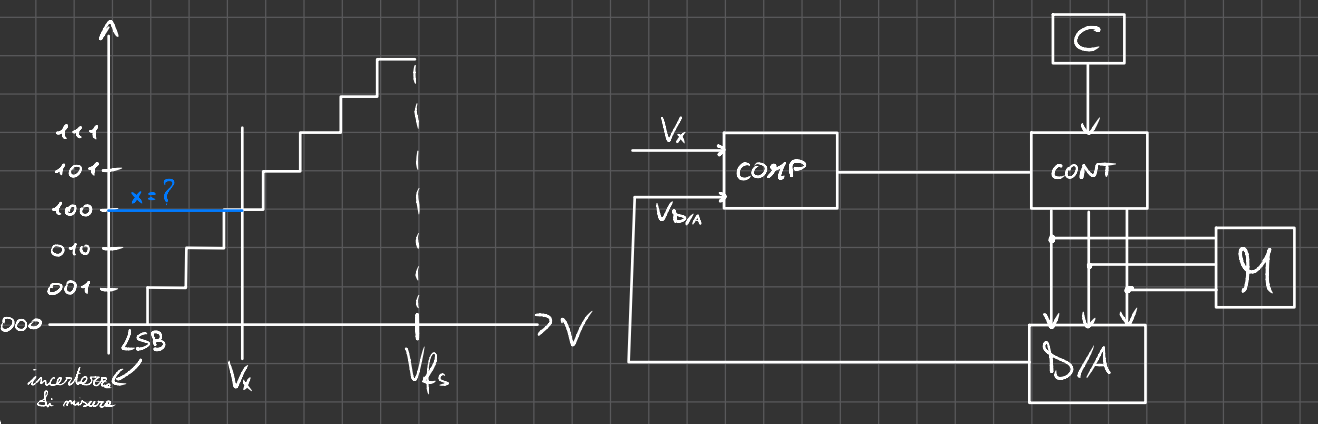
\includegraphics[width=.8\textwidth]{Images/figure28.png}
\end{center}
La linea avrà \textbf{piccole perdite} se:
\begin{itemize}
    \item $\frac{R}{\w L} << 1$\\
    \item $\frac{G}{\w C} << 1$
\end{itemize}
Calcoliamo la \textbf{pulsazione di risonanza fondamentale} e il \textbf{Q} corrispondente:
\begin{equation*}
    \begin{dcases}
    V(z) = - j I(0) Z_0 sin(\beta z)\\
    I(z) = I(0) cos(\beta z)
    \end{dcases}
\end{equation*}
Dove:
\begin{itemize}
    \item $\beta = \w \sqrt{LC}$\\
    \item $Z_0 = \sqrt{\frac{L}{C}}$
\end{itemize}
Quindi:
\begin{equation*}
    \w_0 \sqrt{LC} l = \pi \implies \w_0 = \frac{\pi}{\sqrt{LC} l}
\end{equation*}
Mentre Q sarà:
\begin{equation*}
    Q = \frac{\w_0 W_{EM}}{P_{diss}} = \frac{\w_0 W_{EM}}{P^R_{diss}+ P^G_{diss}} \implies Q = \left(\frac{1}{Q_R} + \frac{1}{Q_G}\right)^{-1}
\end{equation*}
In particolare:
\begin{equation*}
    Q_R = \frac{\w_0 W_{EM}}{P^R_{diss}}, \quad Q_G = \frac{\w_0 W_{EM}}{P^G_{diss}}
\end{equation*}
Dove:
\begin{equation*}
    P^R_{diss} = \frac{1}{2} \int_0^l |I(z)|^2 dz, \quad P^G_{diss} = \frac{1}{2} \int_0^l |V(z)|^2 dz
\end{equation*}.
Quindi:
\begin{equation*}
    W_{EM} = W_M + W_E = \frac{1}{4} L \int_0^l |I(z)|^2 dz + \frac{1}{4} C \int_0^l |V(z)|^2 dz
\end{equation*}
In risonanza $W_E = W_M$, quindi:
\begin{equation*}
    W_{EM} = 2W_M = \frac{1}{2} L \int_0^l |I(z)|^2 dz = \frac{1}{2} C \int_0^l |V(z)|^2 dz = 2W_E
\end{equation*}
Quindi ci\textbf{ semplifichiamo il calcoli} facendo scelte opportune:
\begin{equation*}
    Q_R = \frac{\w_0 \frac{1}{2} L \int_0^l |I(z)|^2 dz}{\frac{1}{2} R \int_0^l |I(z)|^2 dz} = \frac{\w_0 L}{R}
\end{equation*}
\begin{equation*}
    Q_G = \frac{\w_0 \frac{1}{2} C \int_0^l |V(z)|^2 dz}{\frac{1}{2} G \int_0^l |V(z)|^2 dz} = \frac{\w_0 C}{G}
\end{equation*}
Quindi avremo:
\begin{equation*}
    Q = \left(\frac{R}{\w_0 L}  + \frac{G}{\w_0 C}\right)^{-1} = \frac{\w_0 LC}{R C + L G}
\end{equation*}

\subsection{Esempio 2}
Consideriamo la seguente \textbf{linea chiusa su due resistenze, senza perdite}:
\begin{center}
    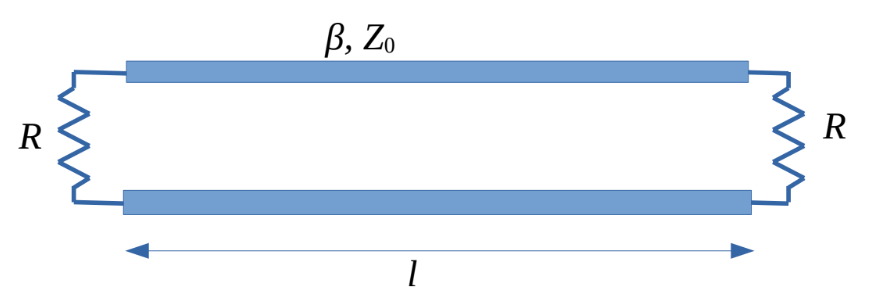
\includegraphics[width=.8\textwidth]{Images/figure29.png}
\end{center}
Suppongo \textbf{R piccole} in modo tale da \textbf{non variare tensioni e correnti sulla linea rispetto al caso 1}.\\ \\
\begin{equation*}
    \begin{dcases}
    V(z) = -j I(0) Z_0 cos(\beta z)\\
    I(z) = I(0) cos(\beta z) 
    \end{dcases}
\end{equation*}
E la \textbf{pulsazione di risonanza} è:
\begin{equation*}
    \w_0\sqrt{LC} l = \pi \implies \w_0 = \frac{\pi}{\sqrt{LC} l }
\end{equation*}
Per calcolare Q ci occorrono l'\textbf{energia immagazzinata e la potenza dissipata}:
\begin{equation*}
    P_{diss} = \frac{1}{2} R |I(0)|^2 + \frac{1}{2} R |I(l)|^2 = R |I(0)|^2
\end{equation*}
\begin{equation*}
\begin{aligned}
    W_{EM} &= 2W_M = \frac{1}{2} L |I(0)|^2 \int_0^l cos^2(\beta z) dz \\
    &(\theta = \beta z \implies dz = \frac{1}{\beta} d\theta)\\
    &\implies \frac{1}{\beta} \int_0^\pi cos^2(\theta) d\theta = \frac{1}{\beta} \int_0^\pi \frac{1}{2} + \frac{1}{2} cos(2\theta) d\theta =\\
    &= \frac{\pi}{2\beta} = \frac{\pi}{2\w_0 \sqrt{LC}} = \frac{\lambda}{4}
\end{aligned}
\end{equation*}
Per cui:
\begin{equation*}
    W_{EM} = \frac{1}{2} L |I(0)|^2 \frac{\pi}{2\w_0 \sqrt{LC}} = \frac{1}{4} \sqrt{\frac{L}{C}} |I(0)|^2 \frac{\pi}{\w_0}
\end{equation*}
Quindi:
\begin{equation*}
    Q = \frac{\w_0 W_{EM}}{P_{diss}} = \frac{\w_0 \frac{1}{4} \sqrt{\frac{L}{C}} |I(0)|^2 \frac{\pi}{\w_0}}{R^2 |I(0)|^2} = \sqrt{\frac{L}{C}} \frac{\pi}{4R} = \frac{\pi}{4} \frac{Z_0}{R}
\end{equation*}
Di conseguenza:
\begin{equation*}
    Q >> 1 \quad se \quad Z_0 >> R
\end{equation*}

\subsection{Esempio 3}
Nel caso in cui $Z_0 << R$, gli andamenti di V e I, sono gli stessi di una \textbf{linea aperta}:
\begin{center}
    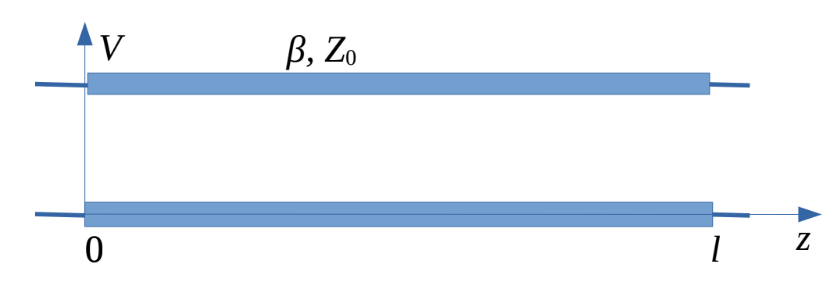
\includegraphics[width=.8\textwidth]{Images/figure30.png}
\end{center}
\begin{equation*}
    \begin{dcases}
    V(z) = V(0) cos(\beta z)\\
    I(z) = -j \frac{V(0)}{Z_0} sin(\beta z)
    \end{dcases}
\end{equation*}
\begin{equation*}
    \w_0 \sqrt{LC} l = \pi \implies \w_0 = \frac{\pi}{\sqrt{LC} l}
\end{equation*}
\begin{equation*}
    P_{diss} = \frac{1}{2} \frac{|V(0)|^2}{R} + \frac{1}{2} \frac{|V(l)|^2}{R} = G|V(0)|^2
\end{equation*}
\begin{equation*}
\begin{aligned}
    W_{EM} &= 2W_E = \frac{1}{2} C |V(0)|^2 \int_0^l cos^2(\beta l) dz = \frac{1}{2} C |V(0)|^2 \frac{\pi}{2\w_0 \sqrt{LC}} = \\
    &=\frac{1}{4} \sqrt{\frac{C}{L}} |V(0)|^2 \frac{\pi}{\w_0}
\end{aligned}
\end{equation*}
Infine:
\begin{equation*}
    Q = \frac{\w_0 W_{EM}}{P_{diss}} = \frac{\w_0 \frac{1}{4} \sqrt{\frac{C}{L}} \frac{\pi}{\w_0}} {G|V(0)|^2} =\sqrt{\frac{C}{L}} \frac{\pi}{4G} = \frac{\pi}{4} \frac{R}{Z_0}
\end{equation*}
Quindi:
\begin{equation*}
    Q >> 1 \quad se \quad Z_0 << R
\end{equation*}

\section{Condizioni di Risonanza su una Rete Complessa}
Consideriamo una rete di \textbf{elementi} \textbf{concentrati} e \textbf{distribuiti} \textbf{senza perdite} e \textbf{senza generatori} e individuiamo una sezione che la divide in due, e alla quale posso inserire un \textbf{generatore di tensione}:
\begin{center}
    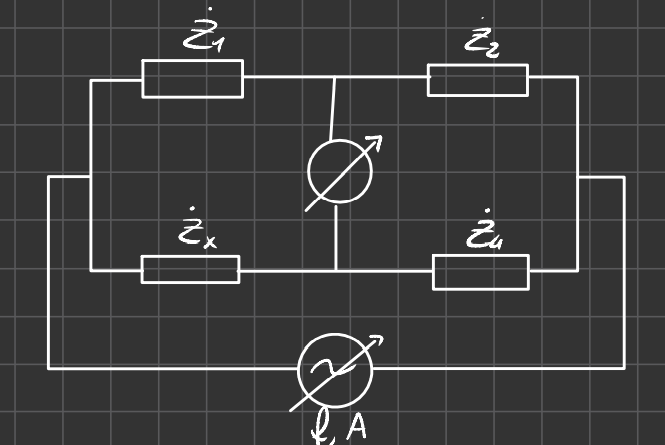
\includegraphics[width=.5\textwidth]{Images/figure31.png}
\end{center}
O di corrente:
\begin{center}
    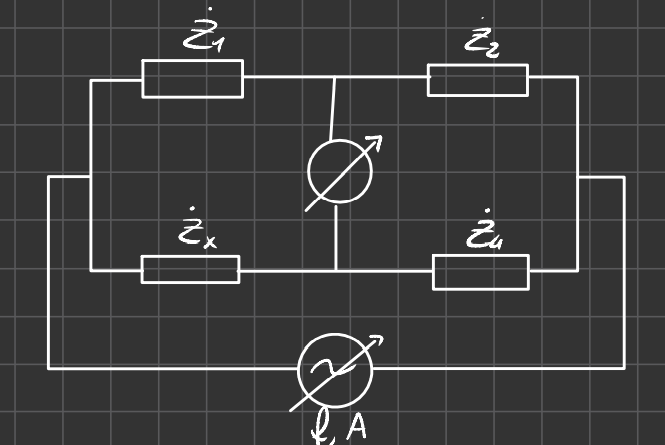
\includegraphics[width=.5\textwidth]{Images/figure31.png}
\end{center}
Nel primo caso:
\begin{equation*}
    I = \frac{V_G}{\overleftarrow{Z}\overrightarrow{Z}}
\end{equation*}
Dove le due impedenze sono pure \textbf{reattanze}.\\ \\
Può accadere che a qualche frequenza $\overleftarrow{Z} + \overrightarrow{Z} = 0$ e nel caso in cui anche $V_G$ fosse 0, queste frequenze vengono dette di \textbf{risonanza}. \\ \\
In modo analogo:
\begin{equation*}
    V = \frac{I_G}{\overleftarrow{Y}\overrightarrow{Y}}
\end{equation*}
Se $\overleftarrow{Y} + \overrightarrow{Y} = 0$ e  $I_G = 0$ sono dette \textbf{frequenze di risonanza}.\\ \\
\begin{center}
    Devono valere entrambe.
\end{center}

\subsection{Esempio 1}
\begin{center}
    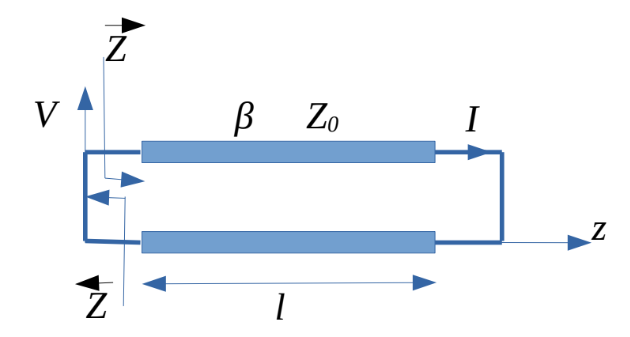
\includegraphics[width=.5\textwidth]{Images/figure33.png}
\end{center}
\begin{equation*}
    \overleftarrow{Z} + \overrightarrow{Z} = 0 + j Z_0 tan(\beta l) = 0
\end{equation*}
\begin{equation*}
    \implies \beta l = n\pi
\end{equation*}
Ma in questo caso:
\begin{equation*}
    \overleftarrow{Y} \longrightarrow \infty
\end{equation*}
\textbf{Quindi non va bene.}
\subsection{Esempio 2}
\begin{center}
    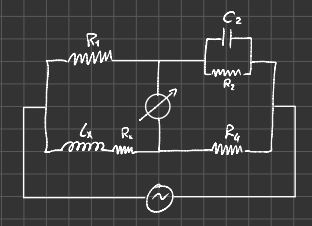
\includegraphics[width=.5\textwidth]{Images/figure34.png}
\end{center}
\begin{equation*}
    \overleftarrow{Z} + \overrightarrow{Z} = j Z_0 tan(\beta l/2) + j Z_0 tan(\beta l/2) = 2 j Z_0 tan(\beta l/2) = 0
\end{equation*}
Le cui soluzioni sono:
\begin{equation*}
    \beta  \frac{l}{2} = \frac{n}{\pi} \leftrightarrow \beta l = 2n\pi \implies l = 2n\frac{\lambda}{2} = n \lambda
\end{equation*}
Mentre per le \textbf{ammettenze}:
\begin{equation*}
    \overleftarrow{Y} + \overrightarrow{Y} = - j Y_0 tan(\beta l/2) - j Y_0 cotan(\beta l/2) = - 2 j Y_0 cotan(\beta l/2) = 0
\end{equation*}
Le cui soluzioni sono:
\begin{equation*}
    \beta  \frac{l}{2} = \frac{\pi}{2} + n\pi \leftrightarrow \beta l = (2n+1) \pi \implies l = (2n+1) \frac{\lambda}{2} 
\end{equation*}
\textbf{Quindi va bene!!}
\chapter{Teorema di Reciprocità}
In un mezzo \textbf{lineare} e \textbf{isotropo}, i campi dovuti a sorgenti diverse sono legati dalla relazione:
\begin{squared}[violet]
    \int_{V_s} \bar{J}_1 \cdot \bar{E}_2 - \bar{J}_2 \cdot \bar{E}_1 dV + \int_{V_s} \bar{J}_{m2} \cdot \bar{H}_1 - \bar{J}_{m1} \cdot \bar{H}_2 dV = 0
\end{squared}
Applichiamo il \textbf{teorema} a un dispositivo con una porta in posizione $\bar{r}_1$ e l'altra in posizione $\bar{r}_2$:
\begin{center}
    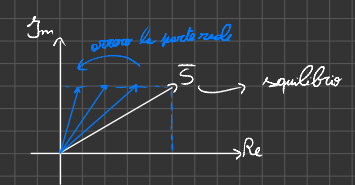
\includegraphics[width=.6\textwidth]{Images/figure35.png}
\end{center}
Dividiamo ora \textbf{due situazioni}:
\begin{center}
    \textbf{(a)}
\end{center}
\begin{center}
    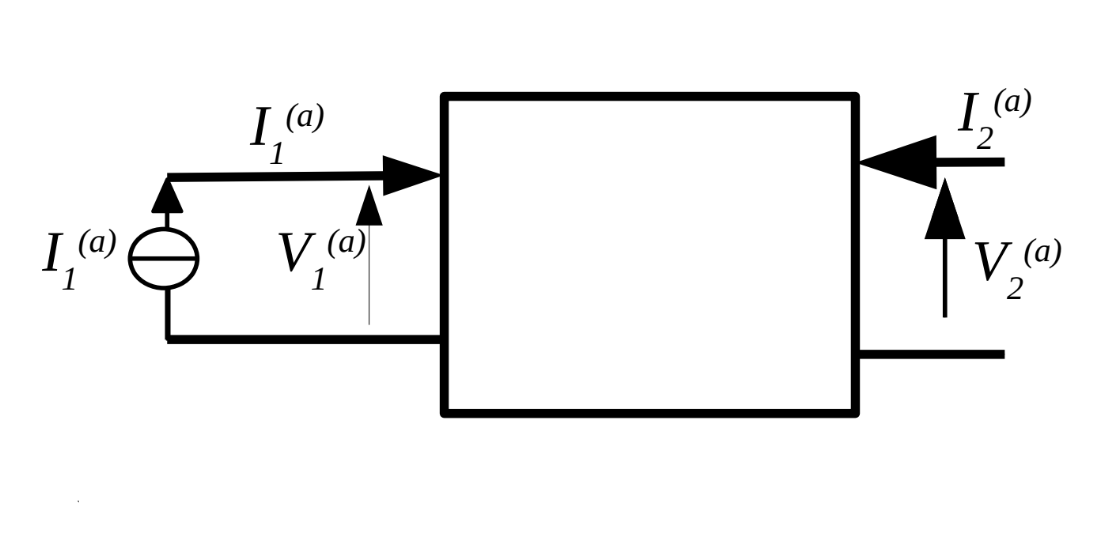
\includegraphics[width=.6\textwidth]{Images/figure36.png}
\end{center}
\begin{equation*}
    \bar{J}_1 = I_1^a \Delta \delta(|\bar{r} - \bar{r}_1|) \hat{i}_1
\end{equation*}
che produce:
\begin{equation*}
    \bar{E}_1 \quad e \quad \bar{H}_1
\end{equation*}

\begin{center}
    \textbf{(b)}
\end{center}
\begin{center}
    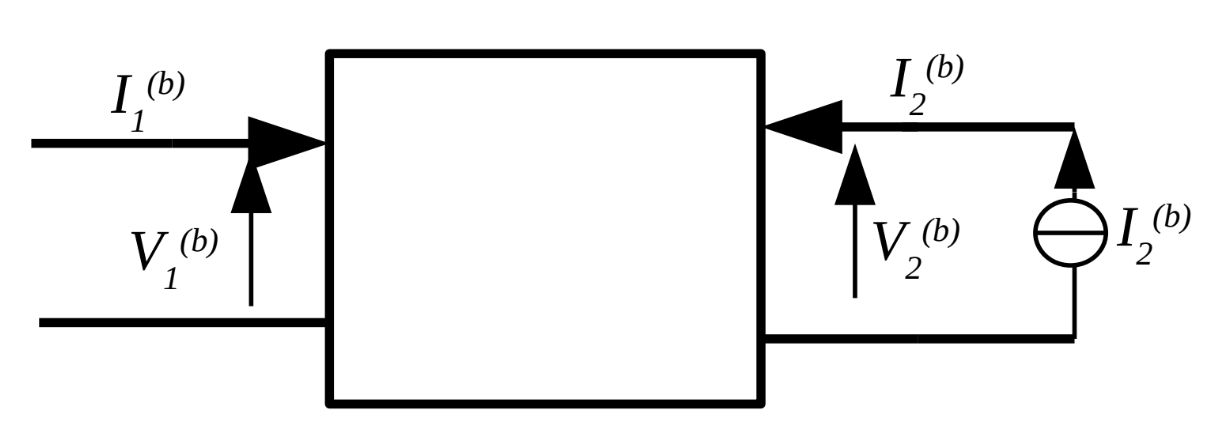
\includegraphics[width=.6\textwidth]{Images/figure37.png}
\end{center}
\begin{equation*}
    \bar{J}_2 = I_2^b \Delta \delta(|\bar{r} - \bar{r}_2|) \hat{i}_2
\end{equation*}
che produce:
\begin{equation*}
    \bar{E}_2 \quad e \quad \bar{H}_2
\end{equation*}
Sostituiamo nella \textbf{tesi}
\begin{equation*}
    \int_{V_s} I_1^a \Delta \delta(|\bar{r} - \bar{r}_1|) \hat{i}_1 \cdot \bar{E}_2 -  I_2^b \Delta \delta(|\bar{r} - \bar{r}_2|) \hat{i}_2 dV = 0
\end{equation*}
Ovvero:
\begin{equation*}
     I_1^a\Delta \int_{V_s}  \delta(|\bar{r} - \bar{r}_1|) \hat{i}_1 \cdot \bar{E}_2 dV =  I_2^b \Delta \int_{V_s}  \delta(|\bar{r} - \bar{r}_2|) \hat{i}_2 dV = 0
\end{equation*}
Che sfruttando la \textbf{proprietà della delta di Dirac} diventa:
\begin{equation*}
\tag{x}
     I_1^a\Delta\hat{i}_1 \bar{E}_2(\bar{r}_1) = I_2^b\Delta\hat{i}_2 \bar{E}_1(\bar{r}_2)
\end{equation*}
Possiamo assumere $\Delta$ \textbf{piccola} rispetto a $\lambda$, quindi possiamo considerare i \textbf{campi costanti} lungo $\Delta$, quindi:
\begin{equation*}
    V_1^b = - \int_{l_1} \bar{E}_2\cdot \hat{i}_1 dl = - \bar{E}_2(\bar{r}_1) \cdot \hat{i}_1 \Delta
\end{equation*}
che rappresenta la tensione alla porta 1 dovuta alla corrente $I_2^b$ alla porta 2.\\ \\
Analogamente:
\begin{equation*}
    V_2^a = - \int_{l_2} \bar{E}_1\cdot \hat{i}_2 dl = - \bar{E}_1(\bar{r}_2) \cdot \hat{i}_2 \Delta
\end{equation*}
Sostituendo in (x) otteniamo:
\begin{squared}
    I_1^a V_1^b = I_2^b V_2^a
\end{squared}












\end{document}
